\documentclass[a4paper, 12pt]{report}
\usepackage{cmap}
\usepackage{amssymb}
\usepackage{amsmath}
\usepackage{graphicx}
\usepackage{amsthm}
\usepackage{upgreek}
\usepackage{setspace}
\usepackage{empheq}
\usepackage{mathtools}
\setcounter{secnumdepth}{5}
\setcounter{tocdepth}{5}
\numberwithin{equation}{section}
\renewcommand{\theequation}{\arabic{equation}}
\usepackage[T2A]{fontenc}
\usepackage[utf8]{inputenc}
\usepackage[normalem]{ulem}
\usepackage{mathtext} % русские буквы в формулах
\usepackage[left=2cm,right=2cm, top=2cm,bottom=2cm,bindingoffset=0cm]{geometry}
\usepackage[english,russian]{babel}
\usepackage[unicode]{hyperref}
\newenvironment{Proof} % имя окружения
{\par\noindent{$\blacklozenge$}} % команды для \begin
{\hfill$\scriptstyle\square$}
\newcommand{\Rm}{\mathbb{R}}
\newcommand{\Cm}{\mathbb{C}}
\newcommand{\Z}{\mathbb{Z}}
\newcommand{\I}{\mathbb{I}}
\newcommand{\N}{\mathbb{N}}
\newcommand{\rank}{\operatorname{rank}}
\newcommand{\Ra}{\Rightarrow}
\newcommand{\ra}{\rightarrow}
\newcommand{\FI}{\Phi}
\newcommand{\Sp}{\text{Sp}}
\newcommand{\ol}{\overline}

\renewcommand{\leq}{\leqslant}
\renewcommand{\geq}{\geqslant}

\renewcommand{\alpha}{\upalpha}
\renewcommand{\beta}{\upbeta}
\renewcommand{\gamma}{\upgamma}
\renewcommand{\delta}{\updelta}
\renewcommand{\varphi}{\upvarphi}
\renewcommand{\phi}{\upvarphi}
\renewcommand{\tau}{\uptau}
\renewcommand{\theta}{\uptheta}
\renewcommand{\eta}{\upeta}
\renewcommand{\lambda}{\uplambda}
\renewcommand{\sigma}{\upsigma}
\renewcommand{\psi}{\uppsi}
\renewcommand{\mu}{\upmu}
\renewcommand{\omega}{\upomega}
\renewcommand{\xi}{\upxi}
\renewcommand{\epsilon}{\upvarepsilon}
\renewcommand{\rho}{\uprho}
\renewcommand{\varepsilon}{\upvarepsilon}

\renewcommand{\d}{\partial}
\renewcommand{\Re}{\operatorname{Re}}
\newcommand{\const}{\operatorname{const}}
\newcommand{\intx}{\int\limits_{x_0}^x}
\newcommand\Norm[1]{\left\| #1 \right\|}
\newcommand{\sumk}{\sum\limits_{k=0}^\infty}
\newcommand{\sumi}{\sum\limits_{i=0}^\infty}
\newtheorem*{theorem}{Теорема}
\newtheorem*{cor}{Следствие}
\newtheorem*{lem}{Лемма}
\title{\textbf{\Huge{Численные методы математической физики}}\\Конспект по 4 курсу 
специальности «прикладная математика»\\(лектор А. М. Будник)}
\date{}
\begin{document}
\maketitle
\tableofcontents{}
\newpage
\section*{Введение.}
В данном курсе мы будем рассматривать задачи математической физики в частных производных. Основной принцип решения состоит в том, что дифференциальное уравнение мы заменяем разностным и ищем приближенное решение на сетке узлов. Такой способ называется \textit{методом конечных разностей} (\textit{методом сеток}). А раздел численных методов, посвященный теории метода конечных разностей, носит название \textit{теория разностных схем}. 
\\\\
Выделим два основных момента при решении:
\begin{enumerate}
\item построение дискретных разностных аппроксимаций для уравнений математической физики и исследование основных характеристик этих аппроксимаций: погрешности, устойчивости и точности разностных схем;
\item решение разностных уравнений прямыми или итерационными методами, которые выбираются из соображений экономичности вычислительного алгоритма.
\end{enumerate}
\chapter{Способы построения и исследования разностных схем.}
\section{Сетки и сеточные функции.}
При численном решении той или иной математической задачи мы не можем воспроизвести приближенное решение для всех значений аргумента. Поэтому в области задания функции выбирается конечное множество точек, и приближенное решение задачи ищется в этих точках.
\\\\
$\bullet$ \textit{Это множество называется \textbf{сеткой}, а отдельные точки этого множества -- \textbf{узлами сетки}.}
\\\\
$\bullet$ \textit{Функция, определенная в узлах сетки, называется \textbf{сеточной функцией}.}
\\\\
Заменяя области непрерывного изменения аргумента сеткой, то есть областью дискретного изменения аргумента, мы осуществляем аппроксимацию пространства решения дифференциального уравнения пространством сеточной функции.
\\\\
\textbf{Пример сетки на отрезке (одномерный случай).}\\\\
В качестве области определения искомой функции мы рассматриваем отрезок на оси $x$.
\begin{enumerate}
\item \textbf{Равномерная сетка.}
Не ограничивая общности, возьмем отрезок $[0,1]$ и разобьем его на $N$ равных частей точками $$x_0=0,\ x_1,\ \ldots,\ x_{N-1},\ x_N=1.$$
Расстояние между соседними точками назовем \textit{шагом сетки} и обозначим его через $h$, а точки $x_i$ примем в качестве \textit{узлов сетки}, $i=\overline{0,N}$. Тогда множество всех $x_i$ составляют \textit{равномерную сетку} на отрезке $[0,1]$, которую будем обозначать следующим образом
$$\overline \omega _ h = \left\{x_i = ih,\ i=\overline{0, N},\ h = \dfrac1N\right\}.$$
\textit{Множество граничных узлов} обозначим как $$\gamma_h = \{x_0, x_N\}.$$
А все остальные точки образуют \textit{множество внутренних узлов}
$$ \omega _ h = \left\{x_i = ih,\ i=\overline{1, N-1},\ h = \dfrac1N\right\}.$$
Таким образом, можно записать 
$$\overline \omega _h = \omega _h \cup \gamma _h.$$
\item \textbf{Неравномерная сетка.}
Возьмем отрезок $[0,1]$ и разобьем его на $N$ частей точками $$0=x_0 < x_1 <\ldots< x_{N-1} < x_N=1.$$
Тогда мы можем записать неравномерную сетку с граничными узлами 
$$\hat {\overline \omega} _ h = \left\{x_i,\ i=\overline{0, N},\ x_0 = 0, \ x_N=1\right\}.$$
Шаг неравномерной сетки зависит от номера узла и удовлетворяет условию нормировки $$\sum_{i=1}^{N} h_i=1,\ \text{где } h_i=x_i - x_{i-1}.$$
Аналогично случаю равномерной сетки можно записать $$\hat {\overline \omega} _ h = \hat \omega_h \cup \hat\gamma _h.$$
\end{enumerate}
\textbf{Пример сетки на плоскости (двумерный случай).}
\begin{enumerate}
\item \textbf{Прямоугольник.} Исходная область прямоугольника $$\overline G = \{(x_1, x_2),\ 0\leq x_\alpha \leq l_\alpha,\ \alpha=1,2\}$$
$$
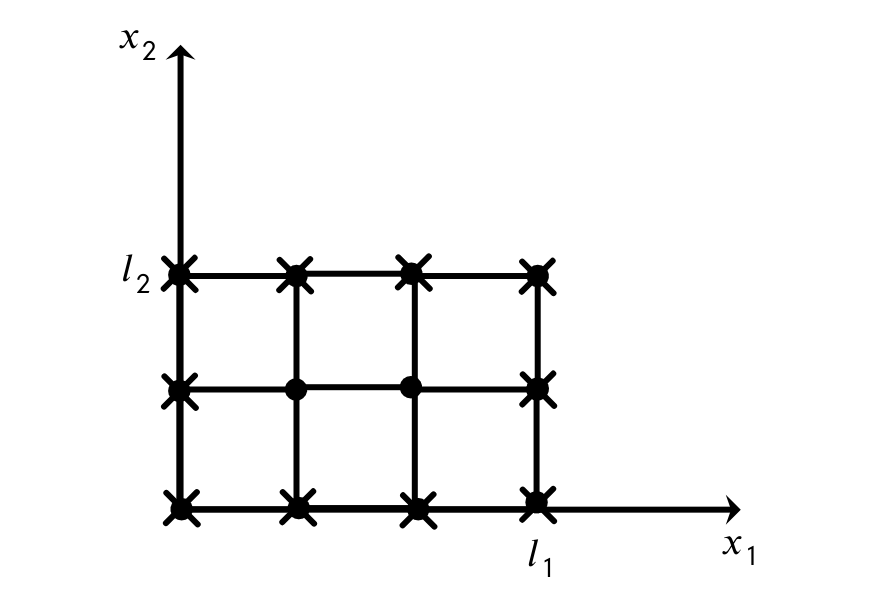
\includegraphics[scale=0.5]{images/img_1}
$$
(кружочками обозначены внутренние узлы, а крестиками -- внешние).\\\\
Сначала построим равномерную сетку. Разобьем отрезки $[0, l_\alpha]$ на $N_\alpha$ частей точками $$0 = x_{\alpha,0} < x_{\alpha, 1} < \ldots < x_{\alpha, N_\alpha -1} < x_{\alpha, N_\alpha} = l_\alpha.$$ Через точки деления проводим прямые, параллельные координатной оси. В качестве узлов двумерной сетки возьмем точки пересечения этих прямых. Общее количество узлов сетки равно $(N_1+1) \times (N_2 + 1)$, а их распределение характеризуется векторным параметром $$h = \{h_{\alpha,1},\ldots, h_{\alpha, N_\alpha},\ h_{\alpha, i_\alpha} = x_{\alpha, i_\alpha} - x_{\alpha, i_\alpha-1},\ i_\alpha = \overline{1, N_\alpha}, \alpha=1,2\}.$$
Тогда \textit{неравномерную двумерную сетку} можно обозначить
$$\hat{ \overline \omega} _ h = \hat{ \overline \omega}_{h_1, h_2} = \hat{ \overline \omega} _ {h_1} \times \hat{ \overline \omega} _ {h_2} = \{(x_{1,i_1}, x_{2, i_2}),\ i_\alpha = \overline{0, N_\alpha},\ x_{\alpha, 0} = 0, x_{\alpha, N_\alpha } = l_\alpha,\ \alpha=1,2\}.$$
Если по каждому направлению шаги сетки равны между собой, то мы получим \textit{двумерную равномерную сетку}
$${ \overline \omega} _ h = { \overline \omega}_{h_1, h_2} =  \overline \omega _ {h_1} \times  \overline \omega _ {h_2} = \left\{(x_{1,i_1}, x_{2, i_2}),\ x_{\alpha, i_\alpha} = i_\alpha h_\alpha,\ i = \overline{0, N_\alpha},\ h_\alpha=\frac{l_\alpha}{N_\alpha},\ \alpha=1,2\right\}.$$
\item \textbf{Область сложной формы.} Пусть нам дана область нерегулярной (сложной) формы $\overline G = G \cup \Gamma$. Для построения сетки мы заключим эту область в прямоугольник $[a,b]\times [c,d]$. В этом прямоугольнике мы строим прямоугольную сетку. Для простоты зададим прямоугольную равномерную сетку. 
$$
	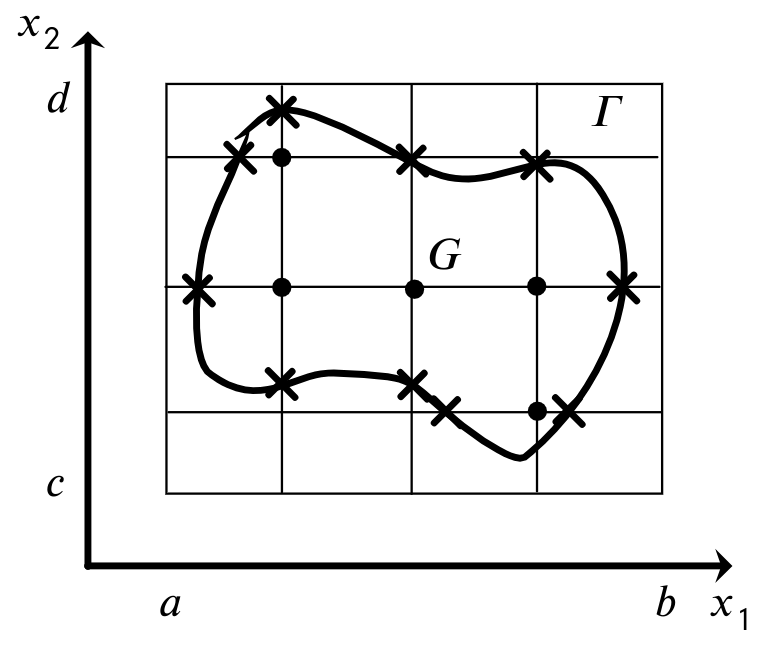
\includegraphics[scale=0.5]{images/img_2}
$$
Те узлы, которые попали внутрь этой сетки, будем считать \textit{внутренними}, обозначим их совокупность $\omega _h$. Точки пересечения прямых $x_\alpha = i_\alpha l_\alpha$, $\alpha=1,2$ с границей $\Gamma$ назовем \textit{граничными узлами}, обозначим их совокупность $\gamma_h$. Тогда сеткой будет множество узлов $$\overline \omega_h = \omega_h \cup \gamma_h$$
Если исходная сетка в прямоугольнике $[a,b]\times [c,d]$ является равномерной, то сетка $\overline\omega_h$ в области $\overline G$ является неравномерной.\\\\
\end{enumerate}
\textbf{Замечания.}
\begin{enumerate}
\item Аналогичным образом строятся сетки и большей размерности. 
\item В зависимости от геометрии исходной области можно использовать и другие ортогональные системы координат.
\item Кроме прямоугольных сеток можно строить, так называемые, треугольные сетки, элементарными ячейками которой являются треугольники. 
\end{enumerate}
Пусть $u(x)$ --- это функция непрерывного аргумента $x = (x_1, \ldots, x_p)\in \overline G$ и $u(x) \in H_0$ ($H_0$ --- функциональное пространство). Если в области $\overline G$ введена сетка $\overline \omega_h$, то вместо функции $u(x)$ можно рассматривать функцию дискретного аргумента $y(x) = y_h$, где $x\in \ol \omega _h$, и эту функцию будем называть \textit{сеточной функцией}, значения которой вычисляются в узлах, а сама функция зависит от шага сетки $h$.\\\\
Множество сеточных функций образует пространство $H_h$ -- \textit{пространство сеточных функций}. Следуя методу конечных разностей, мы заменяем пространство $H_0$ пространством $H_h$. Если $h$ -- параметр, то мы можем рассматривать множество сеточных пространств $\{H_h\}$ для каждого фиксированного $h$.\\\\
Для того, чтобы оперировать функций, нам нужен аппарат для исследования функций и их сравнения. Мы рассматриваем линейные пространства, а для линейных пространств вводится понятие нормы. Соответственно мы определяем \textit{сеточный аналог нормы} $$\Norm {\cdot}_0 \sim \Norm {\cdot} _h.$$
Например, если $H_ 0 = C[0,1]$, то в нем вводится норма $\Norm {\cdot}_0 = \underset{x\in [0,1]} {\max}|u(x)|$. Тогда сеточным аналогом может быть норма $$\Norm {\cdot}_h = \underset{x \in \ol \omega_h}{\max}|y(x)|.$$
Если взять $H_ 0 = L_2[0,1]$, то в нем вводится норма $\Norm {\cdot}_0 = (u,u)^\frac12$. Тогда сеточным аналогом может быть норма $$\Norm {\cdot}_h = \left(\sum_{i=1}^{N-1}hy_i^2\right)^\frac12.$$
Предположим, что функция $u(x)$ -- это решение некоторой дифференциальной задачи. Тогда $y_h(x)$ -- это решение приближенной, или разностной задачи. Для сравнения точного и приближенного решений сеточная функция доопределяется во всех точках области $\ol G$. В результате получается функция непрерывного аргумента $\widetilde{y}_h$, тогда точность решения может быть оценена как $$\Norm{\widetilde{y}_h - u}_0.$$
Другой подход заключается в том, что мы исходное пространство $H_0$ отображаем в пространство $H_h$. Каждой функции $u(x)\in H_0$ ставится в соответствие сеточная функция $u_h(x), x \in \ol \omega _h$, при этом $u_h = P_h u \in H_h$, где $P_h$ -- это линейный оператор проектирования из $H_0$ в $H_h$. Тогда точность решения оценивается как $$\Norm{y-u_h}_h.$$ Для того, чтобы эта операция была корректна, естественно требовать, чтобы норма пространства $H_h$ аппроксимировала норму пространства $H_0$, то есть $$\lim\limits_{h\to 0}\Norm{u_h}_h = \Norm{u}_0.$$
$\bullet$ \textit{Это требование называется \textbf{условием согласованности норм}.}\\\\
\section{Разностная аппроксимация дифференциальных операторов.}
\subsection{Локальная аппроксимация.}
Пусть задан линейный дифференциальный оператор $L$ действующий на функцию $u=u(x)$. Для того, чтобы аппроксимировать (приближенное вычислить) его в любой точке $x\in \omega _h$ разностным оператором $L_h$, необходимо в начале указать или выбрать шаблон $\text {Ш} (x)$. \\\\
$\bullet$ \textit{Под \textbf{шаблоном} $\text{Ш}(x)$ мы понимаем множество узлов сетки, которое будет использоваться при аппроксимации оператора $L$ оператором $L_h$ в точке $x$.}\\\\
$\bullet$ \textit{\textbf{Погрешность аппроксимации дифференциального оператора $L$ разностным оператором $L_h$ в точке $x$} называется величина }
\begin{equation}
\psi(x) = L_hu(x) - Lu(x),\ x\in \omega_h.
\end{equation}
$\bullet$ \textit{Будем говорить, что \textbf{разностный оператор $L_h$ аппроксимирует дифференциальный оператор $L$ с порядком $m>0$ в точке $x$}, если можно представить} $$\psi(x) = O(h^m).$$
Рассмотрим способ построения разностных операторов, получивший название \textit{метод неопределенных коэффициентов}. На выбранном шаблоне $\text{Ш}(x)$ разностную аппроксимацию будем искать в виде линейной комбинации значений функции в точках шаблона \begin{equation}
L_hu(x) = \sum_{\xi \in \text{Ш}(x)} A_h(x, \xi) u(\xi).
\end{equation}
В формуле (2) $A_h(x, \xi)$ -- это неизвестные коэффициенты, выбранные таким образом, чтобы погрешность аппроксимации имела в точке $x$ заданный (чаще всего максимально возможный) порядок. Практический выбор значений коэффициентов осуществляется путем разложения погрешности аппроксимации в ряд Тейлора, то есть мы представляем $$\psi(x) = \sum_{\xi \in \text{Ш}(x)} A_h(x, \xi) u(\xi) - Lu(x),$$
а затем раскладываем получившееся выражение в ряд Тейлора в окрестности точки $x$. После приведения мы получаем в итоге линейную комбинацию 
$$\psi(x) = \sum_{\xi \in \text{Ш}(x)} A_h(x, \xi) u(\xi) - Lu(x) = \sum_{|j|\geq 0} B_h^{(j)}(x) u^{(j)}(x).$$
После этого мы приравниваем к нулю максимально возможное количество первых членов этого разложения. Как правило, количество этих членов совпадает с количеством неизвестных коэффициентов. После этого, решив систему линейных уравнений, находим коэффициенты $A_h$ и по формуле (2) записываем искомый разностный оператор $L_h$.
\\\\
\textbf{Замечания.}
\begin{enumerate}
\item Выбор шаблона зависит от порядка производных, входящих в исходный операторов $L$, а также от требуемой точности аппроксимации.
\item Легко видеть, что для аппроксимации дифференциального оператора, содержащего производную $k$-ого порядка по некоторой переменной, необходимо использовать шаблон, содержащий не менее $(k+1)$ точку вдоль координатного направления соответствующей переменной.
\item Метод неопределенных коэффициентов является не единственным способом построения разностных операторов. Известен в литературе также метод \textit{численного дифференцирования}.
\end{enumerate}
\textbf{Пример 1.}
Пусть задан дифференциальный оператор $$Lu(x) = \dfrac{d u(x)}{dx} = u'(x).$$
\begin{enumerate}
\item Пусть нам дан шаблон $\text{Ш}(x) = \{x, x+h\}$. Тогда по формуле (2) составляем линейную комбинацию
$$u(x) = a_0 u(x) + a_1u(x+h).$$
Записываем выражение для погрешности аппроксимации
$$\psi(x)= a_0u(x) + a_1u(x+h) - u'(x).$$
Затем производим разложение выражения в ряд Тейлора в окрестности точки $x$ и приводим подобные при значениях функции и ее производных
$$\psi(x)= a_0u(x) + a_1u(x+h) - u'(x) = \underbrace{(a_0+a_1)}_{B ^{(0)}}u(x) + \underbrace{(ha_1 - 1)}_{B^{(1)}} u'(x) + \dfrac{h^2}{2} a_1 u''(x) + \ldots.$$
Приравнивая коэффициенты $B^{(j)}$ к нулю, получаем систему линейных уравнений 
$$\begin{cases}
	a_0+a_1 = 0,\\
	ha_1 - 1= 0.
\end{cases}$$
Тогда $$a_0 = -\dfrac 1h,\ a_1 = \dfrac 1h.$$
Таким образом, мы построили разностный оператор вида 
\begin{equation}
	L_hu(x) = \dfrac{u(x+h) - u(x)}{h} = u_x
\end{equation}
$\bullet$ \textit{Обозначение называется \textbf{правой разностной производной}.}\\\\
При этом $$\psi(x) = \dfrac h2 u''(x) + \ldots = O(h),$$ то есть разностный оператор (3) аппроксимирует исходный оператор $L$ с первым порядком.\\\\
$\bullet$ \textit{Величина $\dfrac h 2 u''(x)$ называется \textbf{главным членом погрешности аппроксимации}.}
\item Пусть нам дан шаблон $\text{Ш}(x) = \{x-h, x\}$. Поступая аналогичным образом, мы можем построить оператор вида 
\begin{equation}
	L_hu(x) = \dfrac{u(x) - u(x-h)}{h} = u_{\ol x}
\end{equation}
$\bullet$ \textit{Обозначение $u_{\ol x}$ называется \textbf{левой разностной производной}. }
\\\\
Легко видеть, что $$\psi(x) = -\dfrac h2 u''(x) + \ldots = O(h).$$ 
\item Пусть нам дан шаблон $\text{Ш}(x) = \{x-h, x, x+h\}$. Проделав те же вычисления, мы получим выражение 
\begin{equation}
	L_hu(x) = \dfrac{u(x+h) - u(x-h)}{2h} = u_{\overset\circ x}
\end{equation}
$\bullet$ \textit{Обозначение $u_{\ol x}$ называется \textbf{центральной разностной производной}.}
\\\\
Легко видеть, что $$\psi(x) = -\dfrac {h^2}{6} u'''(x) + O(h^4) = O(h^2).$$ 
\end{enumerate}
Можно заметить, что с увеличением точек шаблона будет также увеличиваться погрешность аппроксимации.\\\\
Можно построить однопараметрическое семейство операторов для аппроксимаиции первой производной следующего вида $$L_h^{(\sigma)}u(x) = \sigma u_x + (1-\sigma)u_{\ol x},$$
где $\sigma$ -- это любое вещественное число. Выражение для погрешности имеет следующий вид
$$\psi(x) = (2\sigma - 1)\dfrac h2 u''(x) + O(h^2).$$
Очевидно, что при любом $\sigma \ne \frac 12$ разностный оператор будет иметь первый порядок аппроксимации $\psi(x) = O(h).$ Иначе мы получаем второй порядок аппроксимации $\psi(x) = O(h^2)$, при этом легко видеть, что $$L_h^{(0,5)} = \dfrac 12(u_x + u_{\ol x}) = u_{\hat x}.$$
\textbf{Пример 2.} Пусть нам дан дифференциальный оператор $$Lu(x) = u''(x).$$ Оператор второго порядка, поэтому для аппроксимации нужно как минимум 3 точки. Возьмем шаблон $\text{Ш}(x) = \{x-h, x, x+h\}$. Применяя метод неопределенных коэффициентов, мы получим следующий разностный оператор \begin{equation}
L_h u(x) = \dfrac{u(x+h) - 2u(x) + u(x-h)}{h^2}=u_{\ol xx}
\end{equation}
$\bullet$ \textit{Обозначение $u_{\ol x x}$ называется \textbf{второй разностной производной}.}\\\\
Погрешность будет иметь вид $$\psi(x) = \dfrac {h^2}{12} u^{IV}(x) + O(h^4) = O(h^2),$$ то есть имеет второй порядок, а не первый, как мы могли ожидать. Оказывается, что именно симметрия шаблона обеспечивает повышение порядка аппроксимации. Но на произвольной сетке мы получили бы первый порядок аппроксимации.\\\\
\textbf{Замечания.}
\begin{enumerate}
	\item Символы, используемые для обозначения разностных производных неслучайны, а является формальными операторами разностного дифференцирования и предписывают, как осуществлять аппроксимации. Например, если мы имеем разностный оператор $u_{\ol x x}$, то можно записать
	\begin{multline*}
		u_{\ol x x} = (u_{\ol x}(x))_x = \dfrac{u_{\ol x}(x+h) - u_{\ol x}(x)}{h} = \dfrac{1}{h}\left(\dfrac{u(x+h) - u(x)}{h} - \dfrac{u(x) - u(x-)}{h}\right) =\\= \dfrac{u(x+h) - 2u(x) - u(x-h)}{h^2}.
	\end{multline*}
	Можно также записывать $$u_{\ol x}(x+h) = u_x(x),\ \dfrac12 (u_x + u_{\ol x}) = u_{ \overset{\circ}{x}}.$$ Соответственно, мы можем конструировать разные операторы. Существуют также и разностные аналоги формул Грина.
	\item Разложение погрешности $\psi(x)$ по степеням $h$ можно использовать для повышения порядка аппроксимации. Например, мы можем заменить четвертую производную четвертой разностной производной в выражении $$u_{\ol x x}(x) - u''(x) = \dfrac{h^2}{12} u^{IV}(x) + O(h^4) = \dfrac{h^2}{12}\left(u_{\ol x x\ol x x}(x) + O(h^2)\right) + O(h^4).$$
	Тогда можно построить разностный оператор $$L_hu(x) = u_{\ol x x}(x) - \dfrac{h^2}{12} u_{\ol x x\ol x x}(x).$$
	Шаблон уже будет $$\text{Ш}(x) = \{x-2h, x-h, x, x+h, x+2h\},$$ а погрешность аппроксимации $$\psi(x) = O(h^4).$$
\end{enumerate}
\textbf{Пример 3.} Пусть дан дифференциальный оператор $$Lu = \dfrac{\d u}{\d t} - \dfrac{\d ^2 u}{\d x ^2},\ u=u(x,t),\ (x,t) \in \omega_{h\tau}.$$
\begin{enumerate}
	\item[(a)] Шаблон может иметь вид $$
		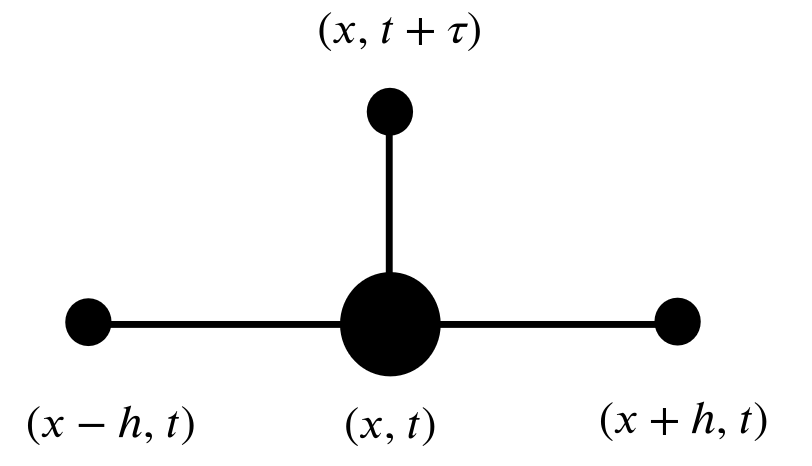
\includegraphics[scale=0.25]{images/img_3}$$
	\item[(b)] Шаблон может иметь вид $$
	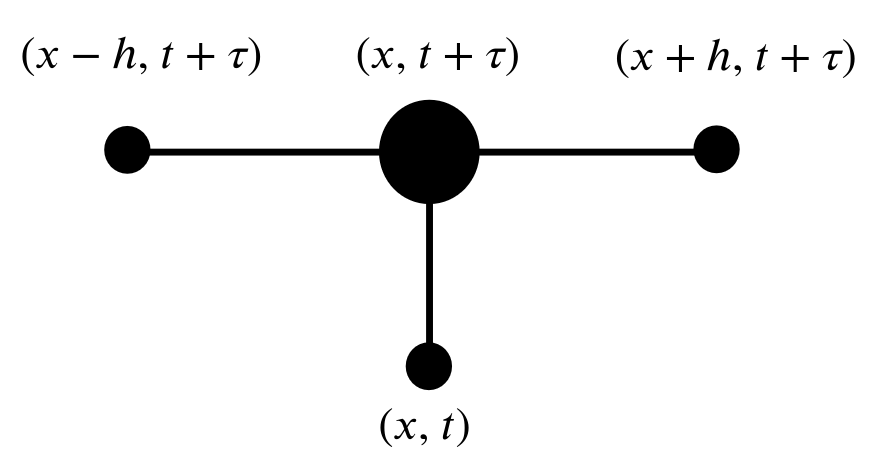
\includegraphics[scale=0.25]{images/img_4}
	$$
	\item[(c)] Шаблон может иметь вид $$
		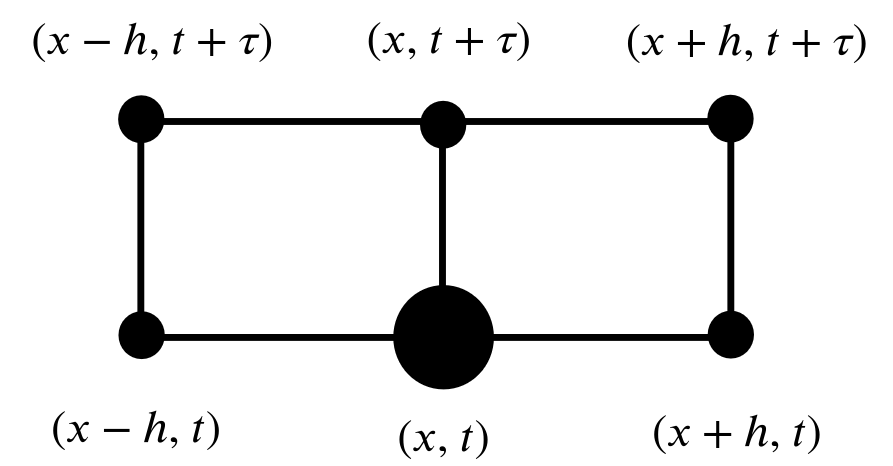
\includegraphics[scale=0.25]{images/img_5}
	$$
\end{enumerate}
Для шаблона (а) мы можем записать оператор $$L_{h\tau} u = \dfrac{u(x, t+\tau) - u(x,t)}{\tau} - \dfrac{u(x+h, t) - 2u(x,t) + u(x-h, t)}{h^2}.$$
Такая форма записи называется \textit{индексной.}
Учитывая введенные обозначения, мы можем записать этот оператор также в форме 
\begin{equation}
	L_{h\tau} u = \dfrac{u(x, t+\tau) - u(x,t)}{\tau} - \dfrac{u(x+h, t) - 2u(x,t) + u(x-h, t)}{h^2} = u_t - u_{\ol x x}.
\end{equation}
Используем следующие обозначения: $$u(x,t) = u,\ u(x, t+\tau) = \hat u, \ u(x, t-\tau) = \check {u}.$$
Тогда для случая (b) можно записать \begin{equation}
	L_{h\tau} u = u_t - \hat u_{\ol x x}.
\end{equation}
Для случая (c) мы можем построить однопараметрическое семейство аппроксимаций вида
\begin{equation}
	L_{h\tau}^{(\sigma)}u = u_{\hat t} - (\sigma \hat u_{\ol x x} - (1-\sigma) u_{\ol x x}),\ \sigma \ne 0,\ \sigma \ne 1.
\end{equation}
Разностный оператор (9) аппроксимирует исходный дифференциальный оператор со вторым порядком по $x$ при любых $\sigma$ и первым порядком по $\tau$ при $\sigma =0, \sigma = 1$. Или вторым порядком по $\tau$ при $\sigma = \dfrac 12$. То есть можно записать записать 
\begin{equation}
	\begin{cases}
		\psi(x,t) = O(\tau + h^2),\ \sigma \ne \dfrac 12,\\
		\psi(x,t) = O(\tau^2 + h^2),\ \sigma = \dfrac 12.
	\end{cases}
\end{equation}
\textbf{Пример 4.} Пусть дан дифференциальный оператор $$Lu = \dfrac{\d ^2u}{\d t^2} - \dfrac{\d ^2 u}{\d x^2}.$$
Сейчас по каждому из направлений у нас будет по 3 точки.
\begin{enumerate}
	\item[(a)] Шаблон может иметь вид 
	$$
		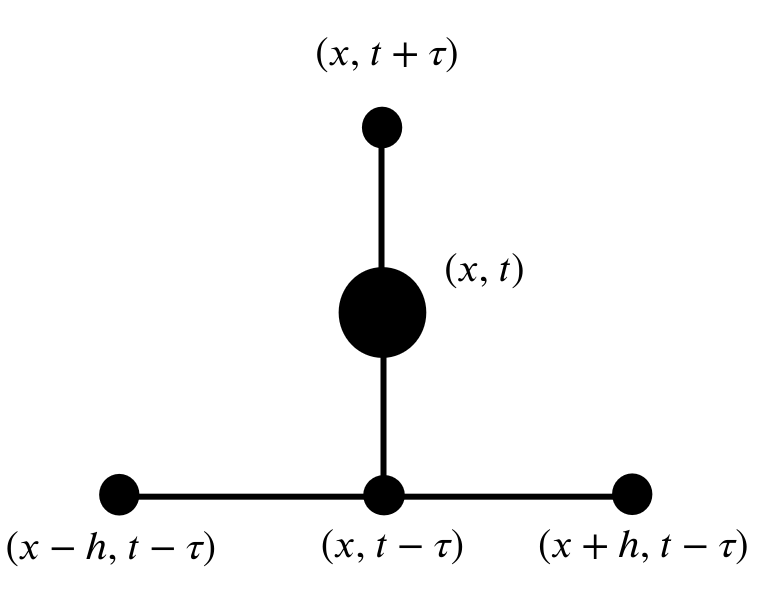
\includegraphics[scale=0.25]{images/img_6}
	$$
	\item[(b)] Шаблон может иметь вид 
	$$
		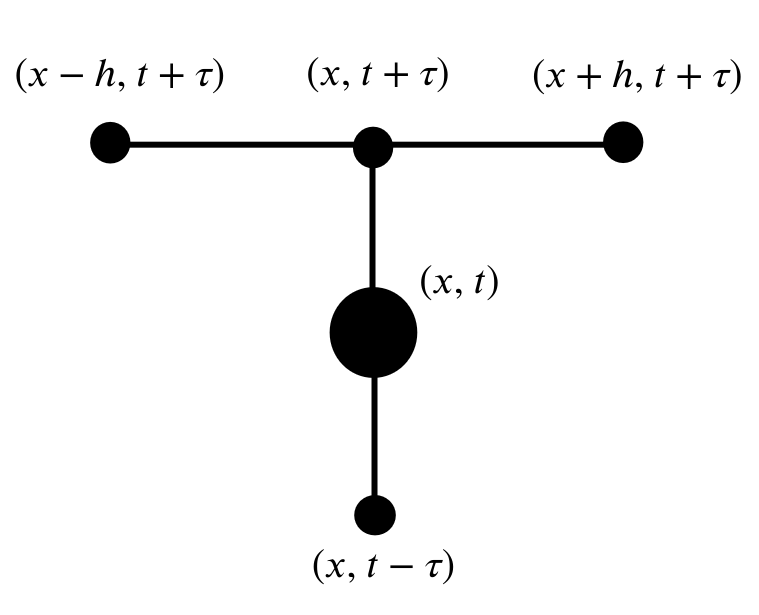
\includegraphics[scale=0.25]{images/img_7}
	$$
	\item[(c)] Шаблон может иметь вид $$
		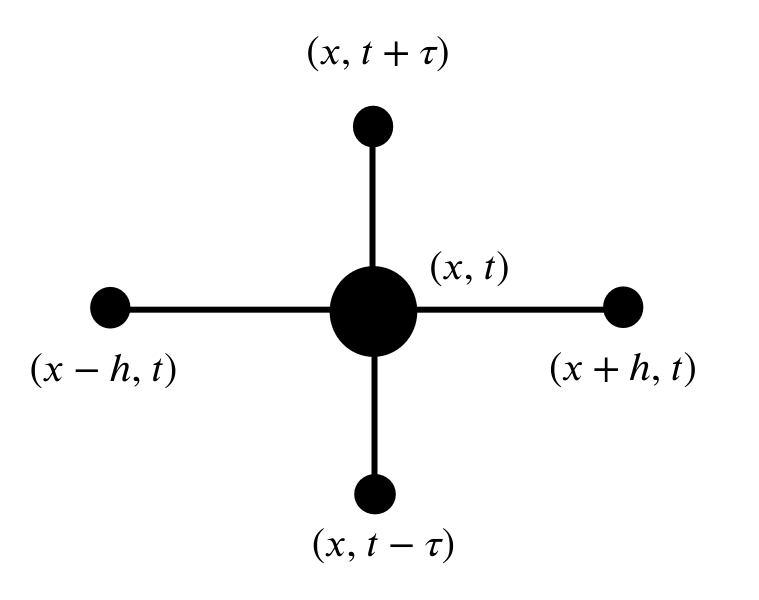
\includegraphics[scale=0.25]{images/img_8}
	$$
	\item[(d)] Шаблон может иметь вид 
	$$
		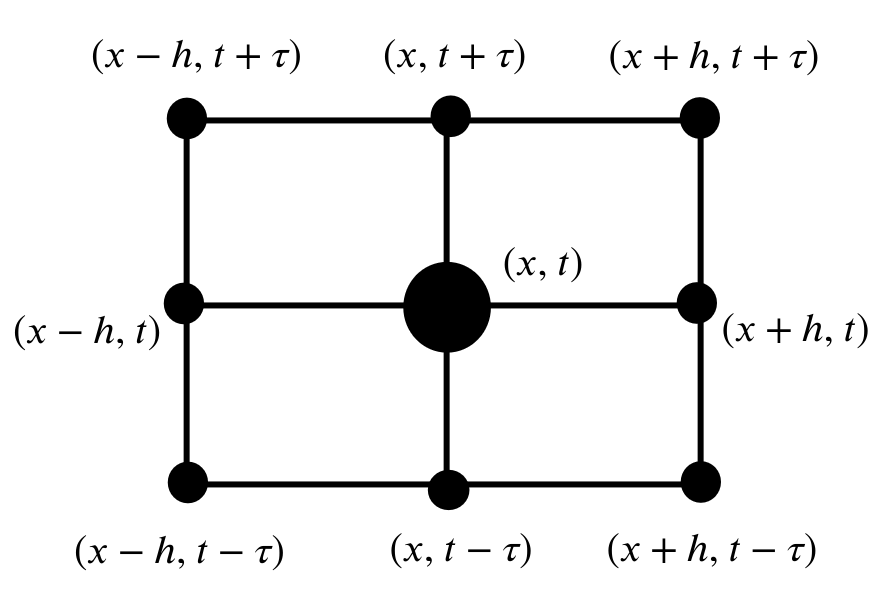
\includegraphics[scale=0.25]{images/img_9}
		$$
\end{enumerate}
Запишем двухпараметрическое семейство для варианта (d)
\begin{equation}
	L_{h\tau}^{(\sigma_1, \sigma_2)}u = u_{\ol t t} - (\sigma_1 \hat u_{\ol x x} + (1-\sigma_1 - \sigma _2) u_{\ol x x} + \sigma_2 \check u_{\ol x x}).
\end{equation}
Для шаблона (а) \begin{equation}
	L_{h\tau}^{(0,1)} u= u_{\ol t t} - \check u_{\ol x x}.
\end{equation}
Для шаблона (b) \begin{equation}
	L_{h\tau}^{(1,0)} u= u_{\ol t t} - \hat u_{\ol x x}.
\end{equation}
Для шаблона (c) \begin{equation}
	L_{h\tau}^{(0,0)} = u_{\ol t t} - u_{\ol x x}.
\end{equation}
Погрешность аппроксимации оператора (14) будет равна $$\psi(x,t) = O(h^2 + \tau^2),\ \sigma_1=\sigma_2 = 0.$$
Если же $\sigma_1 = \sigma_2 = \sigma$, то погрешность будет также иметь второй порядок
$$\psi(x,t) = O(h^2 + \tau^2).$$
Для других значений погрешность аппроксимации по $h$ понижается.
\subsection{Аппроксимация на сетке.}
Ранее мы рассматривали локальную аппроксимацию, то есть аппроксимацию в точке. Сейчас мы рассмотрим основные положения теории разностных схем, касающихся аппроксимации на сетке.\\\\
Пусть $\omega_h$ -- сетка в некоторой области $G$ $p$-мерного пространства, $H_h$ -- линейное пространство сеточных функций, заданных на $\omega_h$, $H_0$ -- пространство гладких функций непрерывного аргумента. В этих пространствах зададим нормы $\Norm{\cdot}_h$ в $H_h$ и $\Norm{\cdot}_0$ в $H_0$ соответственно, согласованные друг с другом, то есть выполняется условие согласованности
$$\lim\limits_{h\to 0}\Norm{u_h}_h = \Norm{u}_0.$$
Для этого должны иметь оператор проектирования $P_h$ такой, чтобы $$P_hu = u_h \in H_h.$$
Этот оператор строится достаточно легко: если $u(x)$ известная в любой точке $x$ из пространства $H_0$, то очевидно мы знаем значения в конкретных точках пространства $H_h$.\\\\
Рассмотрим некоторый оператор $L: H_0 \to H_0$ и наряду с ним оператор $L_h : H \to H$.\\\\
$\bullet$ \textit{Назовем \textbf{погрешностью аппроксимации дифференциального оператора $L$ разностным оператором $L_h$} сеточную функцию}
\begin{equation}
	\psi_h = L_hu - (Lu)_h,
\end{equation}
\textit{где $u_h$ -- это сеточная функция, которая получается за счет проектирования непрерывной функции, то есть $u_h = P_hu$, $(Lu)_h$ -- это действие выбранного оператора проектирования на оператор $Lu$, то есть $(Lu)_h = P_h(Lu)$, $\forall u \in H_0$.	}
Заметим, что выражение для погрешности (15) полностью совпадает с определением погрешности аппроксимации в точке (локальной погрешности), однако здесь мы должны предусмотреть возможность построения такой аппроксимации в любой точки сетки.\\\\
$\bullet$ \textit{Если $$\Norm{\psi_h}\xrightarrow[|h|\to 0]{}0$$ то будем говорить, что \textbf{разностный оператор $L_h$ аппроксимирует дифференциальный оператор $L$ на сетке $\omega_h$}. Если при этом \begin{equation}
		\Norm{\psi_h}_h = \Norm{L_hu_h - (Lu)_h} \leq M \cdot |h|^m,
	\end{equation} где $M$ -- константа, не зависящая от $h$, $m>0$, то будем говорить, что \textbf{разностный оператор $L_h$ аппроксимирует дифференциальный оператор $L$ на сетке $\omega_h$ с порядком $m$.}}
Под модулем $|h|$ мы понимаем следующее.
\begin{enumerate}
	\item Если $h = (h_1,\ldots, h_p)$ -- векторный параметр из $p$-мерного пространства, то $$|h| = \left(h_1^2 + \ldots + h_p^2\right)^\frac12.$$
	При этом возможно, что по каждому из направлений $h_\alpha$, $\alpha = \overline{1,p}$ аппроксимация имеет различный порядок. В таком случае имеет место следующее неравенство
	$$\Norm{\psi_h}_h \leq M \sum_{\alpha=1}^{p}h_\alpha^{m_\alpha},$$
	где $m_\alpha>0$ -- порядок аппроксимации по направлению $h_\alpha$. Взяв в качестве $m = \min (m_1,\ldots, m_p)$, мы можем говорить об общем порядке.
	\item Если $\omega_h$ одномерна и неравномерна. Тогда $h$ будет определяться набором шагов между каждой точкой $$h = (h_1,\ldots, h_N),$$ где $N$ -- это число разбиений. В данном случае $$|h| = \underset{1\leq i \leq N}{\max}h_i.$$
\end{enumerate}
\textbf{Пример 5.} Рассмотрим аппроксимацию оператора $$Lu = u''(x),\ u\in H_0 = C^4[0,1].$$
Случай, когда сетка равномерная, нас не интересует. Построим на отрезке $[0,1]$ неравномерную сетку $$\hat{\ol \omega}_h = \{x_0 < x_1 < \ldots < x_N,\ x_i = x_{i-1}+h_{i},\ i=\ol{1,N},\ x_0=0, x_N=1\}.$$
Итак $h = (h_1,\ldots, h_N)$, где $h_i = x_i - x_{i-1},\ i=\ol{1,N}.$ Для каждого $x_i$, $i=\ol {1, N-1}$ рассмотрим трехточечный шаблон $\{x_{i-1}, x_i, x_{i+1}\}$ и методом неопределенных коэффициентов построим разностный оператор \begin{equation}
	(L_hu)_i = \dfrac{1}{ \hbar_i}\left(\dfrac{u(x_{i+1}) - u(x_i)}{h_{i+1}} - \dfrac{u(x_i) - u(x_{i-1})}{h_i}\right)=u_{\ol x \hat x}.
\end{equation}
В формуле (17) $$\hbar_i = \dfrac12 (h_i + h_{i+1}),\ u_{\hat x}=\dfrac{1}{\hbar_i}(u(x_{i+1}) - u(x_i)).$$
Если будем рассматривать погрешность аппроксимации в каждой точке сетки $x_i$, то получим
$$\psi_i = \dfrac{h_{i+1} - h_i}{3}u''(x_i) + O(\hbar_i^2),\ i = \ol{1, N-1}.$$
Из этого выражения следует, что в сеточной норме $$\Norm{\cdot}_{h, C} = \underset{x \in \hat \omega_h}{\max}|\cdot |$$
норма погрешности равна
$$\Norm{\psi_h}_{h,C} = \underset{1\leq i \leq N}{\max}|\psi_i|=O(h),$$
где $h = \underset{1\leq i \leq N}{\max}h_i.$
Но можно подобрать другую норму, в которой порядок аппроксимации будет другим. Рассмотрим другую норму в пространстве сеточных функций -- \textit{негативную норму}
$$\Norm{\psi_h}_{h, -1}=\sqrt{\sum_{i=1}^{N-1}h_i\left(\sum_{k=1}^i \hbar_k \psi_k\right)^2}.$$
Тогда можно доказать, что величина погрешности в этой норме равна
$$\Norm{\psi_h}_{-1} = O(h^2).$$
Таким образом, исследование локальной погрешности может быть недостаточным для суждения о качестве разностного оператора.
Выбор подходящей нормы всякий раз должен быть предметом изучения. \\\\
Рассмотрим основные нормы, которые мы дальше будем использовать в случае функций двух измерений. Рассмотрим функцию двух аргументов $u(x,t)$, $(x,t) \in G$, и наряду с ней рассмотрим сеточную функцию $y(x,t)$, $x \in \omega_h$, $t \in \omega_\tau$, которая определена на сетке $\omega_{h\tau} = \omega_h \times \omega_\tau$. В сеточном пространстве мы будем рассматривать в основном норму 
$$\Norm{y}_{h\tau} = \underset{t \in \omega_h}{\max}\Norm{y(t)}$$
или 
$$\Norm{y}_{h\tau} = \sqrt{\sum_{t \in \omega_\tau}\tau \Norm{y(t)}_h^2}.$$
\textbf{Пример 6.}
Рассмотрим оператор $$Lu = \dfrac{\d u}{\d t} - \dfrac{\d ^2 u}{\d x ^2},\ u \in H_0 = C^{4,2}[0,1].$$
Возьмем простейшую аппроксимацию
$$L_{h\tau}u = u_t - u_{\ol xx}.$$
Если по $x$ сетка равномерна, то $h$ фиксировано. Распишем оператор в любой точке сетки
$$L_{h\tau}u = u_t - u_{\ol xx} = \dfrac{u_i^{j+1} - u_i^j}{\tau} - \dfrac{u_{i+1}^j - 2u_i^j + u_{i-1}^j}{h^2}.$$
В данном случае в качестве сеточной функции $y$ мы рассматриваем проекцию $u$ на сетку, то есть $u=u(x_i, t_j) = u_i^j$.
Локальная погрешность аппроксимации имеет вид $$L_{h\tau}u - (Lu)_{h\tau} = \psi_{h\tau}(x_i, t_j) = O(\tau + h^2).$$
Легко показать, что данный разностный оператор аппроксимирует исходный оператор на сетке с первым порядком по $t$ и вторым порядком по $x$ в любой из норм, рассматриваемых выше, то есть 
$$\Norm{\psi}_{h\tau} = O(\tau + h^2).$$
Как правило, если мы вычислим погрешность аппроксимации в точке, то она обобщается и на всю сетку.
\section{Разностная аппроксимация дифференциальных задач.}
\subsection{Постановка разностной задачи.}
Как известно, дифференциальная задача включает в себя дифференциальное уравнение и дополнительные условия, которые выделяют из совокупности возможных решений единственное. Поэтому при формулировке разностных задач помимо аппроксимации дифференциальных уравнений, необходимо описывать в разностных уравнениях и дополнительные условия.\\\\
$\bullet$ \textit{Совокупность разностных уравнений, аппроксимирующих дифференциальное уравнение и дополнительные условия, называется \textbf{разностной схемой}.}\\\\
$\bullet$ \textit{Существуют две формы записи разностных схем: \textbf{безиндексная} и \textbf{индексная}.}\\\\
\textbf{Пример 1.} Рассмотрим задачу вида 
\begin{equation}
	\begin{cases}
	u'(t) = f(t),\ t>0,\\
u(0) = u_0 = \const.
\end{cases}
\end{equation}
Для того, чтобы построить разностную схему, необходимо выписать разностное уравнение, которое будет аппроксимировать исходное дифференциальное уравнение. Для начала построим равномерную сетку $$\omega_\tau = \{t_j = j\tau,\ \tau>0,\ j=0,1,\ldots\}.$$
Тогда дифференциальной задаче можно поставить в соответствие разностную схему в \textit{безындексной форме}
\begin{equation}
	\begin{cases}
	y_t = \varphi,\ t \in \omega _t,\\
	y(0) = u_0,
\end{cases}
\end{equation}
или в \textit{индексной форме}
\begin{equation}
	\begin{cases}
		\dfrac{y^{j+1}-y^j}{\tau} = \varphi^i,\ j=0,1,\ldots,\\
		y(0) = u_0,
	\end{cases}
\end{equation}
при этом $$y^j = y(t_j)\approx u(t_j),\ \varphi^j = \varphi(t_j).$$
При этом права часть в разностном уравнении может быть задана различными способами, но при условии выполнения следующего соотношения -- \textit{необходимого условия для обеспечения первого порядка аппроксимации}
$$\varphi - f = O(\tau).$$
Например, в качестве $\varphi$ можно выбирать и $\varphi(t) = f(t)$, $t \in \omega_{\tau}$. Также можно выбирать $$\varphi(t) = \dfrac{f(t) + f(t+\tau)}{2}.$$
После записи разностной схемы необходимо указать способ реализации этой схемы.\\\\ $\bullet$ \textit{\textbf{Под способом реализации} будем понимать построение вычислительного алгоритма, позволяющего найти приближенное решение во всех узлах сетки.}\\\\
В нашем примере способ реализации тривиален. Для способа реализации используется, как правило, индексная форма записи. Запишем алгоритм реализации разностной схемы (2)-(3)
\begin{equation}
	y^{j+1}=y^j + \tau \varphi^j,\ j=0,1,\ldots,\ y^0 = u_0.
\end{equation}
Таким образом, для дифференциальной задачи (1) разностная схема (2)-(3) позволяет найти приближенное решение по алгоритму ее реализации (4).
\\\\
\textbf{Пример 2.}
Рассмотрим задачу для функции двух переменных для уравнения гиперболического типа
\begin{equation}
	\begin{dcases}
		Lu = f(x,t), \ L = \dfrac{\d }{\d t} - \dfrac{\d ^2}{\d x^2},\\
	u = u(x,t),\ 0<x<1,\ 0<t<T,\\
	u(x,0) = u_0(x), \ 0\leq x \leq 1,\\
	u(0,t) = \mu_0(t),\ u(1,t) = \mu_1(t),\ 0\leq t\leq T.
	\end{dcases}
\end{equation}
Для аппроксимации задачи сперва мы должны выписать разностные уравнения, которые определяются приближением соответствующих разностных операторов и заменой непрерывной функции на сеточный аналог. Для простоты построим равномерную по $h$ и $\tau$ сетку узлов
$$\ol \omega_{h\tau} = \ol \omega_h \times \ol \omega_\tau.$$
Выберем шаблон
$$\text{Ш}(x,t) = \{(x-h, t),\ (x,t),\ (x+h,t),\ (x,t+\tau)\},\ x\in \omega_h,\ t \in \omega_\tau.$$
Вместо исходной задачи (5) получим разностную задачу, которая и будет являться разностной схемой в \textit{безындексной форме записи}
\begin{equation}
	\begin{cases}
		y_t = y_{\ol x x} + \varphi,\ \varphi = f+O(\tau + h^2),\ (x,t)\in \omega_{h\tau},\\
	y(x,0) = u_0(x),\ x\in \ol \omega_h,\\
	y(0, t) = \mu_0(t),\ y(1,t) = \mu_1(t),\ t\in \ol\omega_\tau.
	\end{cases}
\end{equation}
Запишем сразу алгоритм реализации этой разностной схемы:
\begin{equation}
	\begin{cases}
	y_i^{j+1} = y_i^j + \tau \left(\dfrac{y_{i+1}^j - 2y_i^j + y_{i-1}^j}{h^2} + \varphi_i^j\right),\ i=\ol{1, N_x-1},\ j=\ol{1, N_t-1},\\
y_i^0 = u_0(x_i),\ i=\ol{0,N_x},\\
y_0^j = \mu_0(t_j),\ y_{N_x}^j = \mu_1(t),\ j=\ol{1, N_t}
\end{cases}
\end{equation}
\subsection{Сходимость и точность разностных схем.}
Пусть дана дифференциальная задача 
\begin{equation}
	Lu = f(x),\ x \in G,
\end{equation}
\begin{equation}
	lu = \mu(x),\ x \in \Gamma.
\end{equation}
Искомая функция $u(x) \in H_0$, $x \in \ol G = G \cup \Gamma$, а $L$, $l$ -- дифференциальные операторы, действующие в пространстве $H_0$ c нормой $\Norm{\cdot}_0$.
Задаче (8)-(9) на сетке $\ol\omega_h = \omega_h \cup \gamma_h$ поставим в соответствие разностную задачу, или разностную схему
\begin{equation}
	L_h y_h = \varphi_h,\ x \in \omega_h
\end{equation}
\begin{equation}
	l_h y_h = \chi _h,\ x \in \gamma_h
\end{equation}
где приближенное решение $y_h(x) \in H_h$, $x \in \ol\omega_h$, а $L_h, l_h$ -- это разностные операторы, дествующие в пространстве $H_h$ с нормой, которая согласована с нормой пространства $H_0$, то есть
$$\lim\limits_{h \to 0}\Norm{\cdot}_h = \Norm{\cdot}_0.$$
$\bullet$ \textit{Разностная задача должна быть \textbf{корректно поставленной}, то есть}
	\begin{enumerate}
		\item \textit{решение $y_h(x)$ задачи $(10)-(11)$ существует и единственно для всех $\varphi_h$, $\chi_h$ из допустимого семейства сеточных функций;}
		\item \textit{решение $y_h(x)$ непрерывно зависит от $\varphi_h$, $\chi_h$, то есть для любого шага сетки $h_0$ существует константа $M$ такая, что при всех $h \leq h_0$ выполняется неравенство $$\Norm{y_h-\widetilde{y}_h}_h \leq M\left(\Norm{\varphi_h - \widetilde{\varphi}_h}_h + \Norm{\chi_h - \widetilde{\chi}_h}_h\right),$$
		где $\widetilde{y}_h$ -- решение задачи $(11)$ с правыми частями $\widetilde{\varphi}_h$, $\widetilde{\chi}_h$. Непрерывная зависимость решений разностной задачи называется \textbf{устойчивостью по входным данным}.}
	\end{enumerate} 
	Факт наличия устойчивости является одним из основных вопросов теории разностных схем.\\\\
	Основной целью всякого приближенного метода является получение решения исходной непрерывной задачи с заданной точностью $\epsilon>0$ за конечное число действий $k$. Поэтому после построения разностной схемы, аппроксимирующей исходную задачу, мы должны убедиться в том, что решение разностной задачи $y_h$ будет являться приближенным значением точного решения задачи $u(x)$.\\\\
	Пусть $u_h$  -- это значения исходной функции $u(x)$ на сетке $\omega_h$. Рассмотрим погрешность разностной схемы (10)-(11). Для этого введем функцию $$z_h = u_h - y_h.$$ Выразим $y_h = u_h - z_h$ и подставим в задачу (10)-(11). Тогда получим задачу для погрешности 
	\begin{equation}
	L_h z_h = \psi_h,\ x \in \omega_h,
	\end{equation}
	\begin{equation}
		l_h z_h = \nu_h,\ x \in \gamma_h,
	\end{equation}
	где
	$$\psi_h = L_h u_h - \varphi_h$$
	$$\nu_h = l_hu_h - \chi_h.$$
	\textit{$\bullet$ Функция $\psi_h$ называется \textbf{погрешностью аппроксимации уравнения $(8)$ разностным уравнением $(10)$}. А функция $\nu_h$ -- \textbf{погрешностью аппроксимации граничных условий $(9)$ разностными граничными условиями $(11)$}.}\\\\
	Для оценки погрешности $z_h$ и погрешности аппроксимации $\psi_h$, $\nu_h$ введем на сеточном множестве функций нормы $\Norm{\cdot}_{1,h}$, $\Norm{\cdot}_{2,h}$, $\Norm{\cdot}_{3,h}$.\\\\
	$\bullet$ \textit{Будем говорить, что решение разностной задачи $(10)-(11)$ \textbf{сходится к решению непрерывной задачи $(8)-(9)$} (что то же самое \textbf{разностная схема $(10)-(11)$ сходится}), если }
	\begin{equation}
		\Norm{z_h}_{1,h}= \Norm{u_h - y_h}_{1,h} \xrightarrow[|h| \to 0]{}0.
	\end{equation}
	\textit{Разностная схема имеет \textbf{$n$-ый порядок точности}, если при достаточно малом $|h|\leq |h_0|$ выполняется неравенство}
	\begin{equation}
		\Norm{z_h}_{1,n}\leq M|h|,
	\end{equation}
	\textit{где $M$ -- константа, не зависящая от $h>0$.}
	\textit{Разностная схема имеет \textbf{$m$-ый порядок аппроксимации}, если} \begin{equation}
		\Norm{\psi_h}_{2,h} = O(|h|^m),\ \Norm{\nu_h}_{3,h} = O(|h|^m).
	\end{equation}
	Обозначим через $f_h$ и $(Lu)_h$ значения правой части уравнения (8) на сетке и значение $Lu$ на сетке. С учетом того, что 
	$$(Lu - f)_h = 0,$$
	то можно общую погрешность аппроксимации уравнения записать в виде
	\begin{equation}
		\psi_h = \psi_h^{(1)} + \psi_h^{(2)},
	\end{equation}
	где
	$$\psi_h^{(1)} = f_h - \varphi_h,$$ -- погрешность аппроксимации правой части
	$$\psi_h^{(2)} = L_h u_h - (Lu)_h,$$ -- погрешность аппроксимации дифференциального оператора. Аналогично можно записать общую погрешность $\nu_h$ и для граничных условий.\\\\
	Оказывается, что понятия сходимости и точности связаны между собой для линейных разностных схем. Зависимость порядка точности от порядка аппроксимации дает теорема Лакса.
	\begin{theorem}
		[Лакса] Если линейная разностная схема устойчива и аппроксимирует исходную дифференциальную задачу, то она сходится. Причем порядок точности схемы определяется порядком ее аппроксимации.
	\end{theorem}
	\subsection{Повышения порядка аппроксимации разностных схем.}
	Поскольку порядок сходимости разностной схемы, а значит и скорость сходимости приближенного решения к точному, зависит от порядка аппроксимации, то вопрос об увеличении порядка аппроксимации без увеличения геометрического шаблона является весьма важным для исследования разностных схем.
	\\\\
	\textbf{Пример 3.} Возьмем задачу и разностную схему из примера 1.
	Рассмотрим погрешность аппроксимации 
	\begin{multline*}
		\psi_\tau(t) = u_t(t) - \varphi(t)= \dfrac{u(t_\tau) - u(t)}{\tau} - \varphi(t) = \left[u(t+\tau) = u(t)+\tau u'(t) + \dfrac{\tau^2}{2}u''(t) + O(\tau^3)\right]=\\ = [u'(t) = f(t),\ u''(t) = f'(t)]=f(t) + \dfrac\tau2 f'(t) - \varphi(t) + O(\tau^2)
	\end{multline*}
	Можно в самом простом случае выбрать $$\varphi(t) = f(t) + O(\tau).$$ Тогда мы получим разностную схему первого порядка $\psi_\tau = O(\tau).$ Причем при таком выборе $\varphi = f$ мы получили \textit{явный метод Эйлера}.\\\\
	Мы также можем взять $$\varphi(t) = f(t) + \dfrac \tau 2 f'(t) + O(\tau^2).$$
	Тогда, если мы свернем
	$$\varphi(t) = f\left(t + \dfrac\tau2\right),$$
	то выражение выше аппроксимируется с порядком $O(\tau^2)$. Подставив это в нашу разностную схему, мы получим схему второго порядка аппроксимации. А это есть ничто иное, как \textit{формула средних прямоугольников}.\\\\
	В качестве $\varphi$ можно выбирать и другие выражения. Например, если выбирать
	$$\varphi = f(t) + \dfrac\tau2 f_t(t),$$ то мы получим \textit{формулу трапеций}.\\\\
	Мы повышали порядок аппроксимации исходя из выбора правой части основного уравнения. Но чаще всего получается так, что задача задается с такими граничными условиями, в которых при минимальном шаблоне понижается порядок аппроксимации. Рассмотрим такой случай
	\\\\
	\textbf{Пример 4.} Рассмотрим третью краевую задачу для обыкновенного дифференциального уравнения следующего вида
	\begin{align}
		&u''(x) - qu(x) = f'(x),\ 0<x<1,\\
		&u'(0) = \sigma_0 u(0) - \mu_0,\\
		&u(1) = \mu_1.
	\end{align}
	В уравнениях (18)-(20) числа $q, \sigma_0, \mu_0, \mu_1$ -- это заданные константы. Построим равномерную сетку $\ol \omega_h = \omega_h \cup \gamma_h$ на отрезке $[0,1]$, где
	$$\omega_h = \left\{x_i = ih,\ i = \ol {1,N-1}, h = \dfrac1N\right\},$$
	$$\gamma_h = \{x_0=0,\ x_N=1\}$$
	Для аппроксимации уравнения (18) выберем шаблон $$\text{Ш}_1(x) = \{x-h, x, x+h\},\ x \in \omega_h.$$
	Для аппроксимации условия (19) выберем шаблон, состоящий из двух точек
	$$\text{Ш}_2(0) = \{x_0, x_1\} = \{0,h\},$$
	Для аппроксимации условия (20) формально выбираем шаблон
	$$\text{Ш}_3(1) = \{x_N\} = \{1\}.$$
	Заменяем дифференциальные производные разностными и строим разностную схему
	\begin{align}
		&y_{\ol x x}(x) - dy(x) = -\varphi(x),\ x\in \omega_h,\\
		&y_x(0) = \sigma_0 y(0) - \mu_0,\\
		&y(1) = \mu_1.
	\end{align}
	Исследуем погрешность аппроксимации. Для любого узла $x \in \omega_h$ запишем величину погрешности как невязку над точным решением
	$$\psi_h = u_{\ol x x} - du + \varphi.$$
	Воспользуемся соотношениями
	$$u_{\ol x x} = u'' + \dfrac{h^2}{12}u^{(IV)} + O(h^4).$$
	Учитывая, что $u'' = qu - f$, получим
	$$\psi_h = qu - f + \dfrac{h^2}{12}u^{(IV)} - du + \varphi + O(h^4) = (q-d)u + (\varphi - f) + O(h^2).$$
	Отсюда видно, что $\psi_h = O(h^2)$, если мы выберем
	$$d = q+ O(h^2),\ \varphi = f + O(h^2),$$ то разностное уравнение (21) будет аппроксимировать исходное разностное уравнение со вторым порядком. \\\\
	Рассмотрим погрешность аппроксимации граничных условий
	\begin{multline*}
		\nu_h(0) = u_x(0) - \sigma_0 u(0) + \mu_0 = u'(0) + \dfrac h2 u''(0) + O(h^2) - \sigma_0 u(0) + \mu_0 =\\= [u'(0) =\sigma_0 u(0) - \mu_0] = \dfrac{h}{2}u''(0) + O(h^2) = O(h).
	\end{multline*}
	Исследуем аппроксимацию второго граничного условия
	$$\nu_h(1) = u(1) - \mu_1 = 0,$$
	то есть условие аппроксимируется точно.\\\\
	В итоге мы получили погрешность аппроксимации граничных условий
	$$\nu_h = \nu_h(0) + \nu_h(1) = O(h),$$ поэтому общий порядок аппроксимации равен сумме порядков аппроксимации
	$$\Psi = \psi_h + \nu_h = O(h).$$
	Следовательно, мы построили схему первого порядка аппроксимации.\\\\
	В данном случае возникает потребность повысить порядок точности схемы, не изменяя размер шаблона. Для этого нам необходимо повысить порядок $\nu_h(0)$. Чтобы добиться этого, введем вместо коэффициентов $\sigma_0$ и $\mu_0$ сеточные коэффициенты $\ol \sigma_0, \ol \mu _0$. Тогда вместо уравнения (22) будем рассматривать уравнение с этими коэффициентами
	\begin{equation}
		y_x(0) = \ol \sigma_0 + \ol \mu _0
	\end{equation}
и подберем эти коэффициенты так, чтобы погрешность аппроксимации была равна $O(h^2)$. Выписываем погрешность аппроксимации с новыми коэффициентами, предполагая, что исходное дифференциальное уравнение (18) выполняется в точке $x =0$.
\begin{multline*}
	 	\nu_h(0) = u_x(0) - \ol\sigma_0 u(0) + \ol\mu_0 = u'(0) - (\ol\sigma_0 u(0) - \ol \mu_0)+ \dfrac h2 u''(0) + O(h^2) =\\= [u''(0) =qu(0) - f(0),\ u'(0)=\sigma_0 u(0) - \mu_0] =\\= \left[\left(\sigma_0 + \dfrac h2 q\right) - \ol\sigma_0\right]u(0) + \left[\ol \mu_0 - \left(\mu_0 + \dfrac h2 f(0)\right)\right] + O(h^2)
\end{multline*}
Если мы выберем
$$\ol \sigma = \sigma_0 + \dfrac h2 q,\ \ol\mu_0 = \mu_0 + \dfrac h2 f(0),$$ то в уравнении (24) мы получим второй порядок аппроксимации, а значит схема (21), (24), (23) будет являться схемой второго порядка аппроксимации.\\\\
	$\bullet$ \textit{Такой способ повышения порядка аппроксимации назвыается \textbf{методом повышения порядка с использованием вида дифференциального оператора}.}\\\\
	\textbf{Пример 5.} Рассмотрим третью краевую задачу для уравнения теплопроводности
	\begin{equation}
		\begin{dcases}
		\dfrac{\d u}{\d t} = \dfrac{\d ^2 u}{\d x^2} + f(x,t),\ 0 < x < 1,\ 0 < t \leq T,\\
		u(x,0) = u_0(x),\ 0 \leq x \leq 1,\\
		\dfrac{\d u(0,t)}{\d x} = \sigma_0 u(0,t) - \mu_0(t),\ 0 \leq t \leq T,\\
		u(1,t) = \mu_1(t),\ 0 \leq t \leq T.
	\end{dcases}
	\end{equation}
	В примере 4 у нас рассматривалась одномерная задача. Здесь же мы рассматриваем двумерную задачу. Ее же мы рассматривали в примере 2 при построении разностных схем.
	\\\\
	Наряду с задачей (25) мы рассмотрим разностную схему (аналогично примеру 2)
	\begin{equation}
		\begin{cases}
			y_t = y_{\ol x x} + \varphi(x,t),\ (x,t) \in \omega_{h\tau},\\
		y(x,0) = u_0(x),\ x \in \ol\omega_h,\\
		y_x(0, t) = \overline{\sigma_0} y(0,t) - \ol \mu_0 (t),\ t \in \o \omega_\tau,\\
		y(1,t) = \mu_1(t),\ t \in \ol \omega_\tau.
		\end{cases}
	\end{equation}
	Здесь мы опускаем моменты задания сетки и построения разностных уравнений. Перед нами стоит задача построить на минимальном шаблоне схему второго порядка аппроксимации по пространственной переменной и первого порядка по временной переменной $$\Psi = O(h^2+\tau).$$
	Для аппроксимации исходного уравнения с заданным порядком нам достаточно в выбрать $$\varphi(x,t) = f(x,t) + O(h^2 + \tau).$$
	Если мы в разностной схеме (26) возьмем $$\ol \sigma_0=\sigma_0,\ \ol \mu_0 = \mu_0(t),$$
	то получим погрешность аппроксимации первого граничного условия
	$$\nu(0,t) = O(h).$$
	Следовательно, общий порядок аппроксимации по пространственной переменной -- первый. А значит мы должны подобрать $\ol \sigma_0, \ol \mu_0(t)$ так, чтобы погрешность аппроксимации была $O(h^2)$. \\\\
	Исследуем погрешность аппроксимации, для этого рассмотрим невязку над точным решением
	\begin{multline*}
		\nu(0,t) = u_x(0,t) - \ol \sigma_0 u(0,t) + \ol \mu_0(t) = \dfrac{\d u(0,t)}{\d x} + \dfrac h2 \dfrac{\d ^2 u(0,t)}{\d x^2} + O(h^2) - \ol \sigma_0 u(0,t) + \ol \mu_0(t) =\\=\left[\dfrac{\d u(0,t)}{\d x} = \sigma_0 u(0,t) - \mu_0(t),\ \dfrac{\d ^2 u(0,t)}{\d x^2}  = \dfrac{\d u (0,t)}{\d t} - f(0,t),\  \dfrac{\d u (0,t)}{\d t} = u_{\ol t}(0,t) + O(\tau)\right]=\\= (\sigma_0 - \ol \sigma_0) u(0,t) + \left(\ol \mu_0(t) - \mu_0(t) + \dfrac{h}{2} u_{\ol t}(0,t) - \dfrac h2 f(0,t)\right) + O(h^2 + h\tau).
	\end{multline*}
	Таким образом, если выбрать 
	\begin{equation}
		\ol \sigma_0 = \sigma_0,\ \ol \mu_0(t) = \mu_0(t) - \dfrac h2 y_{\ol t}(0,t) + \dfrac h2 f(0,t),
	\end{equation}
	то порядок схемы (26) будет повышен и погрешность аппроксимации будет $O(h^2 + \tau).$ Для аппроксимации производной по $t$ мы можем использовать одну из трех известных нам аппроксимаций. Но если бы мы взяли центральную производную, то у нас бы уже увеличился исходный шаблон, то есть нарушено условие минимальности шаблона. Мы взяли левостороннюю аппроксимацию, потому что иначе мы бы не смогли реализовать разностную схему. Чтобы это показать, запишем алгоритм реализации разностной схемы (26)-(27) в индексном виде
	\begin{equation}
		\begin{dcases}
			y_{i}^{j+1} = y_i^j + \dfrac{\tau}{h^2} (y_{i+1}^j - 2y_i^j + y_{i-1}^j) + \tau \varphi_i^j,\ i = \overline {1, N_x - 1},\ j = \overline {0, N_t -1},\\
			y_i^0 = u_0(x),\ i = \overline {0, N_x},\\
			y_0^{j+1} = \dfrac{1}{\frac 1h + \frac{h}{2\tau} + \sigma_0}\left(\dfrac 1h y_1^{j+1} + \dfrac{h}{2\tau}y_0^{j} + \mu_0(t_{j+1}) + \dfrac h2 f(0, t_{j+1})\right),\ j = \overline{0, N_t - 1},\\
			y_{N_t}^{j+1} = \mu_1(t_{j+1}),\ j = \overline{0, N_t - 1}.
		\end{dcases}
	\end{equation}
	Расчеты следует вести следующим образом. В нулевой момент времени используется вторая формула для заполнения нулевого слоя. Затем заполняется первый слой, начиная с левого граничного узла по третьей формуле, но нам нужно знать $y_1^{j+1}$. Поэтому сначала считаются внутренние узлы по первой формуле. После этого уже считаем по третьей формуле левое граничное условие. А затем вычисляется правое граничное условие по четвертой формуле.\\\\
	Для повышения порядка аппроксимации использован прием изменения направления дифференцирования,который позволил вторую производную по $x$ заменить первой производной по $t$.
	\section{Способы построения разностных схем.}
	В первых трех параграфах мы рассмотрели основные понятия теории разностных схем: что такое аппроксимация, что такое сходимость, как строить схемы самым простейшим способом, как повышать порядок аппроксимации за счет замены дифференциальных производных разностными аналогами. Но этот простейший способ аппроксимации не всегда является самым лучшим. Вообще говоря, сам процесс построения разностных схем не может ограничиваться только простейшими аналогами дифференциальных производных.\\\\
	Рассмотрим два подхода, которые применяются для получения разностных схем с разными свойствами, обеспечивающих получение приближенного решения на сетке. Для того, чтобы строить разностные схемы нам нужны некоторые требования, предъявляемые к получаемым разностным схемам.
	\subsection{Требования предъявляемые к разностным схемам.}
	Пусть у нас есть уравнение
	$$Lu(x) = u''(x) - q(x) u(x) = -f(x).$$
	На трехточечном шаблоне мы можем построить двухпараметрчиеское семейство разностных аппроксимаций
	$$L_hy(x_i) = \dfrac{y_{i+1} - 2y_i + y_{i-1}}{h^2} - d_iy_i = -\varphi_i,$$
	где в качестве коэффициентов разностного уравнения мы выбрали не $q(x)$ и $f(x)$, а $d_i$ и $\varphi_i$.
	Для обеспечения соответствующего порядка аппроксимации мы можем выбрать в качестве $d_i$, $\varphi_i$ значения функций $q$ и $f$ в трех точках шаблона
	$$d_i = \alpha q_{i-1} + (1-2\alpha)q_i + \alpha q_{i+1},$$
	$$\varphi_i = \beta f_{i-1} + (1-2\beta)f_i + \beta f_{i+1},$$
	где $\alpha$ и $\beta$ -- некоторые параметры.
	Можно показать, что при любых $\alpha$, $\beta\in \mathbb R$ разностный оператор $L_hy$ будет аппроксимировать исходный оператор $Lu$ со вторым порядком. При этом к коэффициентам $d_i$ и $\varphi_i$ можно без нарушения порядка аппроксимации добавлять слагаемые вида $Ch^2$, $C = \const$. Таким образом, возникает задача выбора разностных схем из множества допустимых заданных на выбранном шаблоне, имеющих один и тот же порядок аппроксимации.\\\\
	Поэтому к любому способу построения той или иной разностной схемы предъявляются определенные требования: \textit{количественные} и \textit{качественные}. Если говорить о количественных требованиях, то можно выделить три основных требования:
		\begin{enumerate}
			\item разностные схемы должны иметь определенный порядок аппроксимации на заданном подмножестве $K' \subset K$ из класса $K$ решаемых задач;
			\item максимальный порядок точности на всем классе $K$ решаемых задач;
			\item минимум операций при машинной реализации решений разностных уравнений, -- \textit{требование экономичности разностных схем}.
		\end{enumerate}
		Выделим также три качественных характеристики:
		\begin{enumerate}
			\item система разностных уравнений должна быть \textit{разрешимой} на любой допустимой сетке и для любой задачи из рассматриваемого класса $K$;
			\item схема должна быть \textit{сходящейся} для любой задачи из рассматриваемого класса $K$;
			\item схема должна быть \textit{однородной}, то есть разностные уравнения для любой задачи из рассматриваемого класса $K$ должны записываться единообразно по одному и тому же закону.
		\end{enumerate}
		Для того, чтобы обеспечить выполнение этих требований, мы рассмотрим два способа построения разностных схем. 
		\subsection{Интегро-интерполяционный метод построения разностных схем (метод баланса).}
		Данный метод позволяет построить разностные схемы, которые получили название \textit{консервативных разностных схем}, то есть таких разностных схем, которые выражают физические законы сохранения на сетке. Проиллюстрируем данный метод на примере задачи для одномерного уравнения теплопроводности вида
		\begin{equation}
			(k(x) u'(x))' - q(x)u(x) = -f(x), \ 0<x<1.
		\end{equation}
		Уравнение (1) описывает процесс стационарного распределения тепла в стержне единичной длины.
		При этом $u(x)$ -- это температура стержня, $k(x)\geq k_0 > 0$ -- коэффициент теплопроводности материала стержня, $q(x)u(x)$ -- это слагаемое, которое отвечает за мощность стоков или источников тепла ($q>0$ -- сток, $q<0$ -- источник), а правая часть $f(x)$ -- это плотность распределения внешних источников или стоков тепла ($f>0$ -- источник, $f<0$ -- сток). \\\\
		Для того, чтобы задача была математически замкнута, нам нужно на концах стержня задать граничные условия. Зададим на концах стержня условия третьего рода
		\begin{equation}
			k(0) u'(0) = \kappa_0 u(0) - g_0,
		\end{equation}
		\begin{equation}
			- k(1) u'(1) = \kappa_1 u(1) - g_1.
		\end{equation}
		В условиях $(2)$ и $(3)$ значения $\kappa_0, \kappa_1, g_0, g_1$ -- заданные константы, которые задают величину и структуру теплового потока на концах стержня.
		Теперь мы желаем построить разностную схему. 
		\subsubsection{Вывод разностных уравнений.}
		Чтобы получить разностную схему, нам нужно получить систему разностных уравнений, которая будет давать возможность найти приближенное решение на заданной сетке. \\\\
		Проинтегрируем исходное уравнение (1) по переменной $x$, $0<x^{(1)}\leq x \leq x^{(2)}<1$:
		$$\int\limits_{x^{(1)}}^{x^{(2)}} (ku')'dx - \int\limits_{x^{(1)}}^{x^{(2)}} q(x)u(x)dx = - \int\limits_{x^{(1)}}^{x^{(2)}} f(x)dx.$$
		Обозначим функцию
		$$W(x) = -k(x) u'(x),$$ которая имеет конкретный физический смысл: $W(x)$ -- это тепловой поток. Таким образом, можно записать
		\begin{equation}
			W(x^{(1)}) - W(x^{(2)})=\int\limits_{x^{(1)}}^{x^{(2)}} (q(x)u(x) - f(x))dx
		\end{equation} 
		$\bullet$ \textit{Уравнение $(4)$ называется \textbf{уравнением баланса}, и оно определяет закон сохранения тепла на отрезке $[x^{(1)}, x^{(2)}]$.}\\\\
		Исходя из уравнения (4) мы будем строить нашу разностную схему, которая будет удовлетворять данному уравнению.
		Пусть на отрезке $[0,1]$ задана равномерная сетка
		$$\ol \omega_h = \left\{x_i = ih,\ i = \overline{0,N}, \ h = \dfrac 1N\right\}.$$
		Обозначим  полуцелые узлы через $$x_{i\pm\frac 12} = x_i \pm \dfrac h2.$$
		На отрезке $[x_{i - \frac 12}, x_{i+\frac 12}]$ запишем уравнение (4) в следующем виде:
		\begin{equation}
			W_{i-\frac 12} - W_{i +\frac 12} - \int\limits_{x_{i-\frac12}}^{x_{i+\frac12}} q(x)u(x)dx  =  - \int\limits_{x_{i-\frac12}}^{x_{i+\frac12}}f(x)dx.
		\end{equation}
		Заменим функцию $u(x)$ на отрезке интегрирования $[x_{i - \frac 12}, x_{i+\frac 12}]$ многочленом нулевой степени, то есть $u(x) \approx P_0(x) = u(x_i) = u_i$. Тогда
		$$\int\limits_{x_{i-\frac12}}^{x_{i+\frac12}} q(x)u(x)dx \approx hd_i u_i,$$
		где через $d_i$ мы обозначили 
		\begin{equation}
			d_i =\dfrac 1h \int\limits_{x_{i-\frac12}}^{x_{i+\frac12}} q(x) dx.
		\end{equation}
		Рассмотрим уравнение (5). Нам нужно вычислить $W$. Для этого, учитывая, что 
		$$-u'(x) = \dfrac{W(x)}{k(x)},$$
		получим
		$$\int\limits_{x_{i-1}}^{x_i} u'(x)dx = \int\limits_{x_{i-1}}^{x_i} \dfrac{W (x)}{k(x)}dx.$$
		Следовательно,
		$$u_{i-1}-u_i = \int\limits_{x_{i-1}}^{x_i} \dfrac{W(x)}{k(x)}dx.$$
		Теперь попробуем вычислить интеграл справа. Для этого заменим $W(x)$ на отрезке $[x_{i-1}, x_i]$ полиномом нулевой степени
		$$W(x) \approx \widetilde P_0(x) = W(x_{i-\frac12}) = W_{i-\frac12}.$$
		Тогда из последнего равенства можем получим
		\begin{equation}
			W_{i-\frac12} \approx -a_i u_{\ol x, i},
		\end{equation}
		где \begin{equation}
			a_i = \left[ \dfrac 1h \int\limits_{x_{i-1}}^{x_i} \dfrac{1}{k(x)}dx\right]^{-1}.
		\end{equation}
		Интеграл от $f(x)$ в уравнении (5) тоже переобозначим и пронормируем
		\begin{equation}
			\varphi_i = \dfrac{1}{h} \int\limits_{x_{i-\frac12}}^{x_{i+\frac12}}f(x)dx
		\end{equation}
		С учетом сделанных обозначений вместо уравнения (5) получим уравнение баланса в новом виде
		$$a_{i+1}u_{\overline x, i+1} - a_i u_{\ol x, i} - h_i d_i u_i\approx -h \varphi_i$$
		Разделив последнее равенство на $h$ и переходя к точному равенству для приближенных значений решения в узлах сетки, получим уравнение баланса в индексной форме
		\begin{equation}
			\dfrac{1}{h}\left(a_{i+1}\dfrac{y_{i+1} - y_i}{h} - a_i \dfrac{y_i - y_{i-1}}{h}\right)-d_iy_i = -\varphi_i,\ i=\overline {1,N-1}
		\end{equation}
		Это же уравнение мы можем записать в безиндексной форме
		\begin{equation}
			(a y_{\ol x})_x - dy = -\varphi,\ x \in \omega_h
		\end{equation}
		В уравнении (11) коэффициенты $a_i$, $d_i$, $\varphi_i$ вычисляются по формулам (8), (6) и (9). Таким образом, мы получили разностное уравнение (10), которое аппроксимирует исходное уравнение (1) во всех внутренних узлах сетки. Для того, чтобы аппроксимировать всю задачу, необходимо аппроксимировать граничные условия (2) и (3).\\\\
		Для начала рассмотрим граничное условие на левой границе. Чтобы его аппроксимировать, запишем уравнение баланса (4) на отрезке $\left[0, \dfrac h2 \right]$. В итоге уравнение баланса (4) превратится в уравнение вида
		\begin{equation}
			W_0 - W_{\frac12} -\int\limits_{0}^{\frac12} q(x)u(x)dx = -\int\limits_{0}^{\frac12} f(x) dx.
		\end{equation} 
		Воспользуемся тем фактом, что
		$$W_0 = -k(0)u'(0),$$
		а по условию (2) мы получим, что
		$$W_0 = -k(0)u'(0) = -\kappa_0 u(0) + g_0.$$
		Из формулы (7) следует, что при $i=1$, получим
		$$W_{\frac 12} = -a_1 u_{\ol x, 1} = -a_1 u_{x,0}.$$
		Для преобразования интеграла будем действовать таким же образом, как и раньше: функцию $u(x)$ заменим полиномом нулевой степени и в качестве константы возьмем левую границу отрезка, то есть $u(x)\approx u(x_0)$. С учетом сделанных вычислений, переходя от функции $u$ к сеточной функции $y$, вместо уравнения (2) получим
		\begin{equation}
			a_1 y_{x,0} = \left(\kappa_0 + \dfrac h2 d_0\right)y_0 - \left(g_0 + \dfrac h2 \varphi_0\right),
		\end{equation}
		где \begin{equation}
			d_0 = \dfrac2h \int\limits_0^{\frac h2}q(x)dx,\ \varphi_0 = \dfrac 2h \int\limits_0^{\frac h2}f(x)dx.
		\end{equation}
		Аналогично можно получить аппроксимацию правого краевого условия. Запишем ее без вывода
		\begin{equation}
			-a_N y_{\ol x, N} = \left(\kappa_1 + \dfrac h2 d_N\right)y_N - \left(g_1 + \dfrac h2 \varphi_N\right),
		\end{equation}
		где
		\begin{equation}
			d_N = \dfrac2h \int\limits_{1-\frac h2}^1 q(x)dx,\ \varphi_N = \dfrac 2h \int\limits_{1-\frac h2}^1f(x)dx.
		\end{equation}
		Таким образом, методом баланса мы построили разностную схему (11), (13), (15)
		$$\begin{dcases}
			(a y_{\ol x})_x - dy = -\varphi,\ x \in \omega_h, \\
			a_1 y_{x,0} = \left(\kappa_0 + \dfrac h2 d_0\right)y_0 - \left(g_0 + \dfrac h2 \varphi_0\right),\\
			-a_N y_{\ol x, N} = \left(\kappa_1 + \dfrac h2 d_N\right)y_N - \left(g_1 + \dfrac h2 \varphi_N\right).
		\end{dcases}$$
		Разностная задача может быть решена методом прогонки, который будет устойчив.\\\\
		Теперь мы должны ответить на вопрос, каков порядок аппроксимации этой разностной схемы.
		\subsubsection{Исследование погрешности аппроксимации.}
		Чтобы установить порядок погрешности аппроксимации разностной схемы (11), (13), (15), необходимо исследовать величину невязки разностных уравнений над точным решением в соответствии с определением погрешности аппроксимации.\\\\
		Рассмотрим первое уравнение (11) и исследуем величину погрешности в любой точке $x_i$, где $x_i$ -- внутренний узел
		$$\psi(x_i) = 	\dfrac{1}{h}\left(a_{i+1}\dfrac{u_{i+1} - u_i}{h} - a_i \dfrac{u_i - u_{i-1}}{h}\right)-d_iy_i + \varphi_i,\ i = \overline {1, N-1}.$$
		Разложив все функции в ряд Тейлора в окрестности точки $x_i$ и пользуясь тем фактом, что в каждой точке $x_i$
		$$(k_i u'_i)' - q_i u_i + f_i = 0,$$
		получим \textit{достаточные условия второго порядка аппроксимации} разностного уравнения (11)
		\begin{equation}
			\dfrac{a_{i+1} - a_i}{h} = k'(x_i) + O(h^2),\ \dfrac{a_{i+1} - a_i}{2} = k(x_i) + O(h^2),
		\end{equation}
		\begin{equation}
			d_i = q(x_i) + O(h^2),
		\end{equation}
		\begin{equation}
			\varphi_i = f(x_i) + O(h^2).
		\end{equation}
		Эти условия получены без предположения о том, что разностные уравнения выводились из условия баланса. Когда мы строили разностную схему, коэффициенты удовлетворяли равенствам (8), (6) и (9). Значит, если мы строим консервативную схему, то коэффициенты должны определяться по этим формулам. С другой стороны, чтобы схема была второго порядка, нам нужно, чтобы коэффициенты удовлетворяли равенствам выше. Поэтому мы докажем, что если коэффициенты вычисляются через интегралы (8), (6) и (9), то условия (17), (18) и (19) будут выполняться. Для доказательства выполнения условия (17) обозначим $$v(x) = \dfrac 1{k(x)}.$$
		Тогда из формулы (8) получим, применяя формулу средних прямоугольников,
		$$\dfrac 1 {a_i} = \dfrac 1h \int\limits_{x_i-1}^{x_i}v(x)dx = v(x_{i-\frac 12}) + \dfrac {h^2}{12}v''(x_{i-\frac 12}) + O(h^4),$$
		а тогда
		$$a_i = k_{i-\frac 12}-\dfrac {h^2}{12}
		\cdot \dfrac {v''(x_{i-\frac12})}{v^2(x_{i-\frac12})} + O(h^4) = k_{i - \frac 12} - \dfrac{h^2}{12} \dfrac{v_i''}{v_i^2} + O(h^3).$$
		Тогда, чтобы доказать выполнение условий (17), составим отношения
		$$\dfrac{a_{i+1} - a_i}{h} = \dfrac{ k_{i+\frac 12} - k_{i - \frac 12}}{h} + O(h^2) = k_i' + O(h^2).$$
		$$\dfrac{a_{i+1} + a_i} 2 = \dfrac{k_{i + \frac 12} + k_{i - \frac 12} - \dfrac {h^2}6 \dfrac {v_i''}{v_i^2} + O(h^3)}{2}= k_i + O(h^2).$$
		Таким образом, оба условия из (17) выполнены, если выбирать коэффициенты $a_i$ по формулам (8). \\\\
		Гораздо проще проверяются условия (18) и (19). Они будут выполнены в силу того, что замена интегралов значениями $q_i$ и $f_i$ соответствует их приближенному вычислению по формуле средних прямоугольников.\\\\
		Итак мы установили, что во всех внутренних узлах погрешность аппроксимации равна $O(h^2)$. И если мы будем вычислять коэффициенты по формулам (8), (6) и (9), то схема будет обладать вторым порядком аппроксимации. \\\\
		Но нам также надо исследовать погрешность аппроксимации граничных условий. Рассмотрим погрешность аппроксимации на левой границе
		$$\nu_1(0) = a_1 u_{x,0} - \left(\kappa_0 + \dfrac h2 d_0\right)u_0 + \left(g_0 + \dfrac h2 \varphi_0\right).$$
		Действует аналогично предыдущему случаю, используя следующее соотношение
		$$a_1 u_{x,0} = a_1 u_{\ol x, 1} = - W_{\frac 12} + O(h^2) = - W_0 - \dfrac h2 W_0' + O(h^2) = k(0)u'(0) + \dfrac h2 (k(0)u'(0))' + O(h^2).$$
		Теперь воспользуемся тем, что по условию (2)
		$$k(0)u'(0) - \kappa_0 u(0) + g_0 = 0,$$
		тогда
		$$n_1(0) = \dfrac h2\left((k(0)u'(0))' - d_0 u(0)+\varphi_0\right) + O(h^2) = \dfrac h2 \Big( (q(0) - d_0)u(0) + (\varphi_0 - f(0))\Big) + O(h^2).$$
		Отсюда мы получаем условия, достаточные для аппроксимации со вторым порядком в точке $x=0$:
		\begin{equation}
			d_ 0 =q(0) + O(h), \ \varphi_0 =f(0) + O(h)
		\end{equation}
		Видно, что условие выполняется, если мы вычисляем значения коэффициентов по формулам (14). Аналогично можно показать, что 
		$$\nu_2(1) = O(h^2),$$
		если
		\begin{equation}
			d_N = q(1) + O(h),\ \varphi_N = f(1) + O(h).
		\end{equation}
		Таким образом, при достаточной гладкости коэффициентов $k$, $q$, $f$ и решения $u$ разностная схема (11), (13), (15) аппроксимирует исходную задачу (1), (2), (3) со вторым порядком.\\\\
		\textbf{Замечание}. При практическом использовании разностной схемы для нахождения ее коэффициентов необязательно вычислять интегралы точно, их можно определять приближенно так, чтобы не нарушались условия (17)-(21).\\\\
		Представление коэффициентов разностной схемы в виде интегралов оказывается полезным в случае разрывных функций $k$, $q$, $f$.
		\subsection{Вариационно-проекционный способ построения разностных схем.}
		\subsubsection{Сущность вариационно-проекционного подхода. Основные термины.}
		Суть вариационного подхода заключается в том, что вместо решения исходной дифференциальной задачи мы рассматриваем эквивалентную ей задачу минимизации функционала, решив которую, то есть найдя минимум функционала, мы получаем искомое решение исходной дифференциальной задачи. С этим подходом мы сталкивались в курсе вычислительных методов алгебры при рассмотрении методов решения линейных систем (итерационные методы вариационного типа), например, методы спуска, невязок, релаксации. В курсе методов численного анализа мы также сталкивались с этим подходом, когда рассматривали краевую задачу для дифференциального уравнения второго порядка, например, методы Ритца и Галеркина.
		\\\\
		Будем рассматривать подход, когда дифференциальная задача сводится к построению приближения $u_n(x)$ к искомой функции $u(x)$ как линейную комбинацию
		$$u_n(x) = \sum_{i=1}^n a_i \varphi_i(x),$$
		где $\varphi_i(x)$ -- базисные функции, а $a_i$ -- это коэффициенты подлежащие определению. Если коэффициенты $a_i$ определяются из условия минимума функционала соответствующего рассматриваемой вариационной задаче, то мы получим, так называемые, \textit{вариационные методы}, среди которых метод Ритца, метод наименьших квадратов. Если определять $a_i$ из условия ортогональности невязки к каждой из базисных функций, то мы придем к, так называемому, \textit{проекционному методу}, среди которых метод Галеркина, метод моментов.\\\\
		Оба эти варианта приводят к системам линейных алгебраических уравнений с \textit{плотной матрицей} (то есть не разреженной, все ее элементы будут ненулевым в общем случае). Чтобы получить систему с \textit{разреженной матрицей}, а значит построить экономичные методы определения приближенного решения, в качестве базисных функций $\varphi_i$ необходимо брать функции с \textit{конечным носителем (финитные функции)}. \textit{Финитные функции} -- это такие функции, которые отличны от нуля лишь на небольшой части той области, где определено искомое решение задачи. При этом такие методы стали называться \textit{вариационно-разностными} либо \textit{проекционно-разностными} в зависимости от способа выбора функционала.
		\\\\
		В заключение отметим, что применение вариационного принципа к решению задач математической физики автоматически приводит к разностным схемам, обладающим свойством консервативности. Это происходит из-за того, что соответствующий функционал, отражающий законы сохранения, достигает своего минимума на решении интересующей нас задачи.
		\subsubsection{Метод Ритца построения разностных схем.}
		Построим вариационно-разностную схему для задачи (1), (2), (3), причем для применения вариационного подхода необходимо потребовать выполнение следующих условий для коэффициентов 
		\begin{equation}
			k(x)\geq k_0 > 0,\ q(x)\geq 0,\ \kappa_0 \geq 0,\ 
		\kappa_1 \geq 0,
		\end{equation}
		чтобы обеспечить возможность применения вариационного подхода.
		Дифференциальная задача (1), (2), (3) при выполнении условий $(22)$ эквивалентна задаче отыскания функции $u(x)$, доставляющей минимум функционала
		\begin{equation}
			J(u) - \dfrac{1}{2}[u,u] - \int\limits_0^1 f(x)u(x)dx - g_0 u(0) - g_1 u(1),
		\end{equation}
		где \begin{equation}
			[u,v] = \int\limits_0^1 (k(x) u'(x)v'(x) + q(x)u(x)v(x))dx + \kappa _0 u(0)v(0) + \kappa_1 u(1)v(1).
		\end{equation}
		Построим последовательность конечномерных подпространств $V_n \in W_2^1[0,1]$ размерности $n$ и будем на этих подпространствах искать минимум функционала $(23)$.
		Базис в каждом подпространстве $V_n$ будем обозначать через $\eta_i^{(n)}$, $i=\overline{0,n-1}$. Тогда любой элемент пространства $u_n \in V_n$ представим в виде линейной комбинации
		\begin{equation}
			u_n = \sum_{i=0}^{n-1} a_i \eta_i^{(n)}.
		\end{equation}
		Коэффициенты $a_0, a_1,\ldots, a_{n-1}$, будем находить из условия минимума функционала. Условие минимума функционала приводит к системе уравнений относительно $a_i$
		\begin{equation}
			\sum_{j=0}^{n-1}\alpha_{ij} a_j = \beta_i,\ i = \overline{0, n-1},
		\end{equation}
		где
		\begin{equation}
			\alpha_{ij} = [\eta_{i}^{(n)}, \eta_j^{(n)}],\ \beta_i = \int\limits_0^1 f(x)\eta_i^{(n)}(x)dx + g_0 \eta_i^{(n)}(0) + g_1 \eta_i^{(n)}(1).
		\end{equation}
		Пусть на отрезке $[0,1]$ задана сетка $$\omega_h = \left\{x_i = ih,\ i = \overline{0,N},\ h = \dfrac 1N\right\},$$
		тогда зададим $N = n-1$. Система (26) будет иметь вид трехточечной разностной схемы, если матрица той системы будет трехдиалогнальной, то есть если коэффициенты $\alpha_{ij} = 0,$ если $|i-j|>1$. Более того мы сразу будем добиваться того, чтобы в качестве параметров разложения (25) были значения функции $u_n$ в узлах сетки $\omega_h$. Матрица системы (26) будет трехдиагональной, если базисные функции подпространства $V_n$ будут ортогональны в смысле скалярного произведения (24) при $|i-j|\geq 2$. Это условие будет выполнено, если в качестве базисных функций $\eta_i^{(N+1)}(x)$ взять функции, которые отличны от нуля, если $|x-x_i| \leq h$, $x \in [0,1]$. Так мы обеспечили первое условие. Второе же условие (совпадения в узлах сетки) обеспечивается равенством $\eta_i^{(N+1)}(x_i) = 1$, то есть построенные базисные функции в узлах сетки равны единице.\\\\
		Опишем самый простейший вариант определения функций $\eta_i^{(N+1)}$:
		\begin{gather}
				\eta_0^{(N+1)}(x) = \begin{cases}
				\dfrac{h-x}{h},\ x \in [0,h],\\
				0,\ x \not \in [0,h];
			\end{cases} \notag \\
			\eta_i^{(N+1)}(x) = \begin{cases}
				\dfrac{x-x_{i-1}}{h},\ x \in [x_{i-1},x_i],\\
				\dfrac{x_{i+1} - x}{h},\ x \in [x_i,x_{i+1}],\\
				0,\ x \not \in [x_{i-1}, x_{i+1}].
			\end{cases}\ i = \overline {1, N-1},\\
			\eta_N^{(N+1)}(x) = \begin{cases}
				\dfrac{x-1+h}{h},\ x \in [1-h, 1],\\
				0,\ x\not \in [1-h, 1].
			\end{cases}\notag
			\end{gather}
		Фактически мы задали базис, чтобы аппроксимировать нашу функцию линейной комбинацией базисных функций.
		$$
			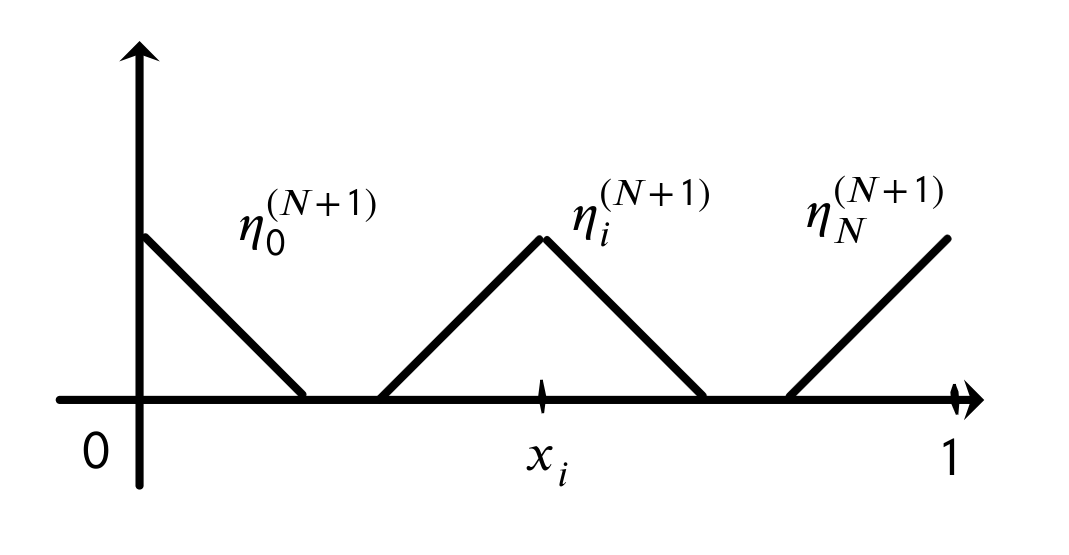
\includegraphics[scale=0.4]{images/img_10}
		$$
		В итоге при подстановке вместо системы (26) мы получим трехдиагональную систему вида
		\begin{equation}
			\begin{cases}
				\alpha_{ii-1} y_{i-1} + \alpha_{ii} y_i + \alpha_{i i+1} y_{i+1} = \beta_i,\ i = \overline {1, N -1},\\
				\alpha_{00} y_0 + \alpha_{01}y_1 = \beta_0,\\
				\alpha_{NN-1} y_{N-1} + \alpha_{NN}y_N = \beta_N,
			\end{cases}
		\end{equation}
		где $y_i \approx u_n(x_i)$, $$\alpha_{ii} = \dfrac{1}{h^2}\left[ \int\limits_{x_{i-1}}^{x_{i+1}} k(x)dx +\int\limits_{x_{i-1}}^{x_i}q(x)(x-x_{i-1})^2dx + \int\limits_{x_i}^{x_{i+1}}q(x)(x_{i+1}-x)^2dx \right],\ i = \overline{1, N-1},$$
		$$\alpha_{ii+1} = \dfrac{1}{h^2} \left[-\int\limits_{x_i}^{x_{i+1}}k(x)dx + \int\limits_{x_i}^{x_{i+1}}q(x)(x-x_i)(x_{i+1} - x)dx\right],\ i = \overline {0, N-1},$$
		причем $\alpha_{ii+1} = \alpha_{i+1i}$. Тогда можно вычислить
		$$\beta_i = \dfrac{1}{h} \left[\int\limits_{x_{i-1}}^{x_i}f(x)(x-x_{i-1})dx + \int\limits_{x_i}^{x_{i+1}}f(x)(x_{i+1}-x)dx\right],\ i = \overline{1, N-1},$$
		$$\alpha_{00} = \dfrac{1}{h^2}\left[\int\limits_0^h k(x)dx + \int\limits_0^h q(x)(x-h)^2dx\right] + \kappa_0,$$
		$$\alpha_{NN} = \dfrac{1}{h^2}\left[\int\limits_{1-h}^h k(x)dx + \int\limits_{1-h}^h q(x)(x-1+h)^2dx\right] + \kappa_1,$$
		$$\beta_0 = \dfrac 1h \left[\int\limits_0^h f(x)(h-x)dx + g_0\right] = \dfrac{1}{h} \int\limits_{1-h}^1 f(x)(x-1+h)dx + g_1.$$
		Систему (29) можно привести к виду (11), (13), (15). При этом у нас получится следующее соотношение между коэффициентами
		$$a_i = - h\alpha_{ii-1},\ d_i = \dfrac 1h (\alpha_{ii-1} + \alpha_{ii} + \alpha_{ii+1}),\ \varphi_i = \dfrac 1h \beta_i,\ i=\overline{1, N-1}.$$
		Аналогично можно преобразовать коэффициенты для граничных условий $d_0, d_N, \varphi_0, \varphi_N$. \\\\
		Можно показать, что вариационно разностная схема, построенная по методу Ритца, является консервативной и обладает вторым порядком аппроксимации. По методу Бубнова-Галеркина аналогичным образом можно построить проекционно-разностные схемы, которые применимы для задач с несамосопряженным оператором, поскольку основным ограничением метода Ритца является достаточно жесткое требование, предъявляемое к исходной задаче: оператор должен быть положительный и самосопряженный. 
		\section{Методы исследования устойчивости разностных схем}
		\subsection{Принцип максимума}
		Этот метод исследования устойчивости позволяет получать равномерные оценки решения через правую часть уравнения, граничные и начальные условия.\\\\
		Пусть $\Omega$ -- это некоторое конечное множество точек $x = (x_1,\ldots, x_p)$ $p$-мерного евклидова пространства. Пусть также в каждой точке $x\in \Omega$ задан шаблон $\text{Ш} (x)\subset \Omega$. Обозначим 
		$$\text{Ш} '(x) = \text{Ш} (x) \backslash \{x\},$$
		окрестность точки $x$. Рассмотрим уравнение 
		\begin{equation}
			Sy(x) = F(x),\ x \in \Omega
		\end{equation}
		где $y(x)$ -- это искомая сеточная функция, $F(x)$ -- это заданная сеточная функция, а $S$ -- это линейный оператор, определяемый следующей формулой
		\begin{equation}
			Sv(x) = A(x)v(x) - \sum_{\xi \in \text{Ш}'(x)} B(x,\xi) v(\xi),
		\end{equation}
		где $v(x)$ -- это любая сеточная функция, коэффициенты $A(x)$, $B(x,\xi)$ -- это заданные сеточные функции. Для определенности будем предполагать, что коэффициенты $A$ и $B$ удовлетворяют условиям :
		\begin{align}
				1.\ A(x) &> 0,\ B(x,\xi) > 0,\ x \in \Omega,\ \xi \in \text{Ш}'(x); \notag\\
				2.\ D(x) &= A(x) - \sum\limits_{\xi \in \text{Ш}'(x)} B(x,\xi)\geq 0.
		\end{align}
		В этих обозначениях уравнение (1) представляем собой разностную схему. Пусть $x$ -- это произвольный узел сетки. Тогда возможны два случая \begin{enumerate}
			\item $\text{Ш}'(x) = \emptyset$;
			\item $\text{Ш}'(x)$ содержит хотя бы один $\xi \in \Omega$.
		\end{enumerate}
		В первом случае уравнение (1) примет простой вид
		$$A(\ol x)y(\ol x) = F(\ol x),$$
		тогда $$y(\ol x) = \dfrac A F = g(x)$$
		и точку $\ol x \in \gamma$ мы будем называть \textit{граничным узлом}. Остальные же узлы, окрестность которых состоит по крайней мере из одной точки (второй случай), будем называть \textit{внутренними узлами}. В итоге из сделанных определений получим, что
		$$\Omega = \omega \cup \gamma$$
		(следует иметь ввиду, что, если мы имеем дифференциальную задачу с краевыми условиями второго или третьего рода, данного определения граничных узлов не существует).\\\\
		Предположим, что сетка $\Omega$ связная.\\\\
		$\bullet$ \textit{Сетка узлов называется \textbf{связной}, если для любых двух узлов $\tilde x, \tilde{\tilde{x}}$, не являющихся одновременно граничными, можно указать такую последовательность узлов $x_1,\ldots, x_m$, что каждый последующий узел принадлежит окрестности предыдущего, то есть} 
		\begin{equation}
			x_1 \in \text{Ш}'(\tilde x), x_2 \in \text{Ш}'(x_1),\ldots, x_m \in \text{Ш}'(x_{m-1}), \tilde{\tilde x} \in \text{Ш}'(x_m).
		\end{equation}
		При сделанных предположениях сформулируем основную теорему
		\begin{theorem}
			[принцип максимума]
			Пусть $y(x)$ -- это отличная от тождественной постоянной сеточная функция определенная на связной сетке $\Omega$ и пусть на $\omega$ выполнены условия $(3)$. Тогда из условия $S y(x) \leq 0$ $(Sy(x) \geq 0)$ на $\omega$ следует, что $y(x)$ не может принимать наибольшего положительного (наименьшего отрицательного) значения во внутренних узлах сетки $\Omega$.
		\end{theorem}
		\begin{Proof}
			Для доказательства теоремы рассмотрим случай $Sy(x) \leq 0$. Доказательство проведем от противного. Предположим, что существует такой узел $\tilde x \in \omega$, в котором $$y(\tilde x) = \underset{x \in \omega}{\max}\ y(x) > 0.$$
			Рассмотрим оператор $$Sy(\tilde x) = D(\tilde x) y(\tilde x) + \sum_{\xi \in \text{Ш}'(\tilde x)} B(\tilde x, \xi) (y(\tilde x) - y(\xi))\geq 0,$$
			 учитывая то, что выполняются условия (3), имеем тот факт, что это выражение положительное. Но с другой стороны по условию теоремы $Sy(\tilde x) \leq 0$. А отсюда следует, что $S y(\tilde x) = 0$. Но, учитывая тот факт, что $D(\tilde x)\geq 0$, $B (\tilde x), \xi) > $, получаем, что $$D(\tilde x) = 0.$$ А значит $$y(\tilde x) = y(\xi),\ \xi \in \text{Ш}'(\tilde x).$$
			 Так как сеточная функция $y(x)$ отлична от тождественной константы, то существует такой узел $\tilde{\tilde x}\in \omega$, что $$y(\tilde{\tilde x})<y(\tilde x).$$
			 В силу связности сетки $\omega$ можно указать последовательность узлов, удовлетворяющую условию (4). Предположим, что $y(x_1) = y(\tilde x)$, тогда 
			 $$y(x_1) = y(x_2) = \ldots = y(x_m) = y(\tilde x).$$
			 Тогда для точки $x_m$ мы получим равенство
			 $$Sy(x_m) = D(x_m) y(x_m) + \sum_{\xi \in \text{Ш}'(x_m)} B(x_m, \xi) (y(x_m) - y(\xi))\geq B(x_m, \tilde{\tilde x}) (y(x_m) - y(\tilde{\tilde x}))> 0,$$
			 то есть существует такая точка, в которой $Sy(x)>0$, что является противоречием с предположением о том, что $Sy(x) \geq 0$. Следовательно, предположение, которое мы сделали о существовании узла $\tilde x$ оказалось неверным, а значит теорема доказана.
		\end{Proof}\\\\
		Сформулируем два следствия к этой теореме.
		\begin{cor}
			Пусть $Sy(x) \leq 0$ ($Sy(x) \geq 0$), $x \in \Omega$, где $\Omega$ -- связная сетка. При этом для оператора $S$ выполняются условия $(3)$. Кроме того существует по крайней мере один узел $x_0 \in \Omega$, для которого \begin{equation}
				D(x_0) > 0.
			\end{equation}
			Тогда $y(x) \leq 0$ ($y(x)\geq 0$) на $\Omega$.
		\end{cor}
		\begin{Proof}
			Без доказательства.
		\end{Proof}
		\begin{cor}
			Пусть оператор $S$ удовтетворя ет увлосвия $(3)$ и $(5)$). Тоггда задача $(1)$-$(2)$ имеет единственное решение.
		\end{cor}
		\begin{Proof}
			Без доказательства.
		\end{Proof}
		\begin{theorem} [сравнения]
			Пусть $y(x)$ -- это решение задачи $(1)$, $(3)$, $(5)$, а $\tilde y(x)$ -- это решение той же задачи, но с другой правой частью $\tilde F (x)$. Тогда из условия, что \begin{equation*}
				|F(x)| \leq \tilde F(x)
			\end{equation*}
			следует, что \begin{equation*}
				|y(x)|\leq \tilde y(x),\ x \in \Omega.
			\end{equation*}
		\end{theorem}
		\begin{Proof}
			Имеем две задачи $Sy(x) = F(x)$, $S \tilde y(x) = \tilde F(x)$. Если сложим обе задачи, то получим, учитывая линейность оператора $S$,
			$$S(y + \tilde y) = F + \tilde F \geq 0.$$
			Если вычтем из первой задачи вторую, то получим
			$$S(y - \tilde y) = F - \tilde F \geq 0.$$
			Из этих неравенств по следствию 1 следует, что $$\begin{cases}
				\tilde y + y \geq 0,\\ \tilde y - y \geq 0.
			\end{cases}$$
			Отсюда следует, что
			$$|y|\leq \tilde y.$$
		\end{Proof}\\
		В качестве мажорантной функции $\tilde F$ обычно можно использовать 
		$$\tilde F = \Norm{F(x)}_C$$
		или
		$$\tilde F = |F(x)|.$$
		Тогда теорема сравнения позволяет сразу получить оценку решения первой краевой задачи в случае однородного уравнения (1). А значит можно сформулировать следующий результат.
		\begin{cor}
			Для решения однородной задачи с краевыми условиями первого рода
			$$\begin{cases}
				Sy(x) = 0,\ x\in \Omega,\\
				y(x) = \mu(x),\ x \in \gamma;
			\end{cases}$$
			справедлива оценка
			$$\underset{x \in \Omega}{\max} |y(x)| \leq |\mu(x)|$$
			или же
			\begin{equation}
				\Norm{y}_C \leq \Norm{\mu}.
			\end{equation}
			Эта оценка является априорной.
		\end{cor}
		\begin{Proof}
			Без доказательства.
		\end{Proof}
		 \begin{theorem}
		 	Если $D(x)>0$ для всех $x \in \Omega$, то для решения задачи $(1)-(3)$ верна априорная оценка
		 	$$\underset{x \in \Omega}{\max}|y(x)| \leq \underset{x \in \Omega}{\max} \dfrac{|F(x)|}{D(x)}$$
		 	или что то же самое
		 	\begin{equation}
		 		\Norm{y}\leq \Norm{\dfrac{F}{D}}
		 	\end{equation}
		 \end{theorem}
		 \begin{Proof}
		 	Доказательство аналогично принципу максимума.
		 \end{Proof}\\\\
		 Сформулируем \textit{алгоритм исследования устойчивости с помощью принципа максимума}.
		 \begin{enumerate}
		 	\item Необходимо привести разностную схему к виду (1)-(2).
		 	\item Проверить условия (3) и (5).
		 	\item Если условия (3) и (5) выполнены, то разностная схема является устойчивой. В противном случае разностная схема не удовлетворяет условиям принципа максимума.
		 \end{enumerate}
		 \textbf{Замечания.}
		 \begin{enumerate}
		 	\item Разностные схемы, коэффициенты которых удовлетворяют условиям принципа максимума при всех значениях параметра $h$ называются \textit{монотонными разностными схемами.}
		 	\item При выполнении условий (3) и (5) следует устойчивость разностной схемы в норме $C$. При этом тип устойчивости определяется тем подмножеством, на котором выполняются условия (5). (дописать с войса)
		 	\item приведение исследуемой разностной схемы к виду (1) следует производить, как правило, так, чтобы коэффициент $A(x)$ был диагональным элементом матрицы при записи задачи в матрично-векторной форме.
		 \end{enumerate}
		 \textbf{Пример.} Рассмотрим задачу Коши для уравнения переноса следующего вида
		 \begin{equation*}
		 	\begin{cases}
		 	\dfrac{\d u}{\d t} + a \dfrac{\d u}{\d x} = 0,\ t>0, -\infty < x < \infty,\ a \equiv \const > 0,\\
		 	u(x,0) = u_0(x).
		 	\end{cases}
		 \end{equation*} Искомая функция $u = u(x,t)$. Прежде, чем исследовать схему на устойчивость, мы должны ее построить. Пройдем все этапы, касающиеся построения и исследования разностной схемы.
		 Чтобы построить схему, нам нужно определить сетку. Определим ее как
		 $$\omega _{h\tau} = \omega_h \times \omega _\tau.$$
		 Далее мы должны выбрать минимальный шаблон. Зададим его следующим образом 
		 $$
		 	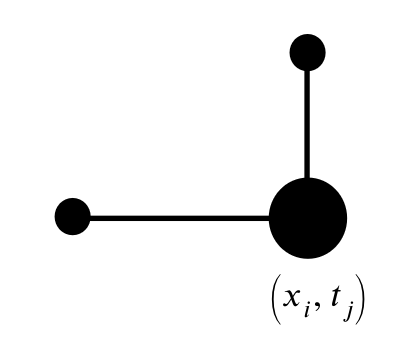
\includegraphics[scale=0.5]{images/img_11}
		 $$
		 Тогда для любой точки сетки мы можем построить разностную схему в бензиднексной форме вида
		 $$\begin{cases}
		 	y_t + a y_{\ol x} = 0,\ x \in \omega_{h\tau},\\
		 	y(x,0) = u_0(x),\ x \in \omega_h,\ t=0.
		 \end{cases}$$
		 с порядком аппроксимации
		 $$\Psi = O(h+\tau).$$
		 Для реализации нужно расписать ее в индексной форме
		 $$\begin{cases}
		 	\dfrac{y_i^{j+1}-y_i^j}{\tau} + a \dfrac{y_i^j - y_{i-1}^j}{h} = 0,\ i =0,\pm1,\ldots,\ j = 0,1,\ldots,\\
		 	y_i^0 = u_0(x_i),\ i =0,\pm1,\ldots.
		 \end{cases}$$
		 В этой схеме единственным неизвестным решением для каждого значения $i, j$ является $y_i^{j+1}$. Следуя алгоритму исследования устойчивости, мы должны привести разностную схему к виду (1)-(2) или, другими словами, определить коэффициенты $A,B,D$.
		 Поэтому мы в качестве точки для исследования устойчивости возьмем точку $(x_i, t_{j+1})$. Таким образом, мы можем переписать аппроксимацию основного уравнения переноса
		 $$\dfrac{1}{\tau} y_i^{j+1} = \left(\dfrac{1}{\tau} - \dfrac a h\right)y_i^j + \dfrac a hy_{i-1}^j.$$
		 Учитывая вид (1)-(2), можем записать, что (считая формально $x = (x_i, t_{j+1})$)
		 $$A(x) = \dfrac 1 \tau,\ B_1 = \dfrac 1 \tau - \dfrac a h,\ B_2 = \dfrac a h,$$
		 $$D(x) = A(x) - (B_1 + B_2) \equiv 0,\ F(x)\equiv 0.$$
		 Мы привели к виду (1)-(2). Теперь мы должны проверить условия (3), (5), получаем
		 $$A(x) = \dfrac 1 \tau > 0, B_1 = \dfrac 1 \tau - \dfrac a h > 0,\ B_2 = \dfrac a h > 0,$$
		 причем второе условие выполняется, когда из условия $B_1 > 0$ следует. что $\frac {a\tau } h < 1$, или, что то же самое, \begin{equation}
		 	\tau < \dfrac h a
		 \end{equation}
		 $\bullet$ \textit{Условие $(8)$ называется \textbf{условием устойчивости Куранта}}.\\\\
		 \textbf{Замечание.} В неравенстве (3) условие для коэффициентов $B$ можно ослабить, то есть рассматривать нестрогое неравенство. Тогда
		 $$B_1 = \dfrac 1 \tau - \dfrac a h \geq 0 \Rightarrow \tau \leq \dfrac h a.$$
		 Если $B=0$, то это означает, что в операторе $(2)$ нет коэффициента в сумме, а значит для данной точки $x$ шаблон не включает эту точку.\\\\
		 В заключение отметим, что при выполнении условия Куранта на основании следствия 3 можно получить оценку разностного решения
		 $$\Norm{y}\leq \Norm{u_0},$$
		 из которой следует устойчивость по начальным данным.
		 \subsection{Метод разделения переменных.}
		 Следуя идее метода разделения переменных будем искать частное решение в виде произведения функций, каждая из которых зависит от одной независимой переменной. В итоге мы придем к задаче на собственные значения для разностного уравнения. И на основании решения задачи на собственные значения, мы можем сделать заключение об устойчивости решения разностной задачи, а следовательно, сделать вывод об устойчивости разностной схемы.\\\\
		 Рассмотрим сеточную функцию $y_h$, определенную на сетке $$\ol \omega _h = \left\{x_k = kh,\ k = \ol{0,N},\ h = \dfrac 1N\right\}.$$
		 Доопределим эту функцию на всей числовой прямой с координатами $x_k = kh$, $(k = 0, \pm 1, \pm 2,\ldots)$ так, чтобы получилась $l$-периодическая сеточная функция. Множество таких функций обозначим через $M_h$. В пространстве $M_h$ введем скалярное произведение
		 $$(v_h, y_h) = \sum_{s=0}^{N-1} h v_h(x_s) y_h(x_s).$$
		 Базисом в этом пространстве будет являться система линейно независимых $l$-периодических функций следующего вида
		 $$\mu_k(x)=\exp\left(ik \frac {2\pi}lx\right),\ i = \sqrt{-1},\ k=0,\pm1,\pm2,\ldots,\pm \dfrac {N-1}{2}\ (k=0,\ldots,N-1).$$
		 Очевидно, что $$(\mu_k(x), \mu_m(x)) = l\cdot \delta ^m_k.$$
		 Следовательно, любую функцию из $M_h$ можно представить как
		 $$y_h(x) = \sum_{k=0}^{N-1} a_k \mu_k(x).$$
		 Заметим, что $\mu_k(x)$ являются собственными функциями операторов правой и левой разностных производных:
		 $$(\mu_k(x))_x = \dfrac{\mu_k(x+h) - \mu_k(x)}{h} = \lambda \mu_k(x),$$
		 тогда $\mu_k(x)$ удовлетворяет условию
		 $$\lambda_k = \dfrac{\exp\left(ik \frac {2\pi}lx\right) - 1}{h}.$$
		 Аналогичный результат у левосторонней разностной производной. Таким образом, функции $\mu_k(x)$ образуют полную систему собственных функций для оператора
		 $L_h$ вида $$L_h y_h = \sum_{s,q} a_{sq}D^s \ol D^q y_h,$$
		 где
		 $$D^s y_h = y_{\underbrace{x\ldots x}_s},\ \ol D^q y_h = y_{\underbrace{\ol x\ldots \ol x}_q}.$$
		 Рассмотрим применение метода разделения переменных к линейным двухслойным разностным схемам, которые записаны в каноническом виде
		 \begin{equation}
		 	By_t + A y = \varphi,
		 \end{equation}
		 где $B, A$ -- это разностные операторы, действующие по по пространственной переменной $x$.\\\\
		 Рассмотрим задачу для погрешности при фиксированной правой части. В этом случае погрешность $z$ приближенного решения будет удовлетворять однородному уравнению
		 \begin{equation}
		 	B \hat z = (B - \tau A)z,
		 \end{equation} 
		 где $\hat z$ -- это погрешность на $(j+1)$-ом временном слое. Будем искать частное решение уравнения (10) в виде
		 \begin{equation}
		 	z_k(x_s, t_j) = q_k^j \exp \left(ik \frac {2\pi}lx_s\right).
		 \end{equation}
		 Из последней формулы следует, что
		 $$\hat z_k = q_kz_k,$$
		 где $q_k$ -- это множитель роста $k$-ой гармоники при переходе с одного временного слоя на другой. Подставляя (11) в (10) и предполагая, что у каждой разностной схемы постоянные коэффициенты, получим формулы для определения $q_k$:
		 $$q_k^{j+1}\lambda _k(B)  \exp \left(ik \frac {2\pi}lx_s\right) = q_k^j (\lambda _k (B) - \tau \lambda_k (A)) \exp \left(ik \frac {2\pi}lx_s\right),$$
		 откуда
		 $$q_k = 1 - \tau \dfrac{\lambda _k( A)}{\lambda_k (B)}.$$
		 \begin{theorem}
		 	[признак устойчивости]
		 	Разностная схема $(9)$ устойчива по начальным данным, если для всех $x$ выполняется неравенство
		 	\begin{equation}
		 		|q_k| \leq 1 + c\tau,
		 	\end{equation}
		 	где $c = \const$, не зависящая от шагов сетки $h$ и $\tau$
		 	(под модулем понимается модуль комплексного числа).
		 \end{theorem}
		 \begin{Proof}
		 	Разложим произвольную ошибку начальных данных по системе базисных функций $\mu_k(x)$
		 	$$z(x_s, t_0) = \sum_{k=0}^{N-1}a_k \exp \left(ik \frac {2\pi}lx_s\right).$$
		 	В силу линейности можем записать
		 	$$z(x_s, t_j) = \sum_{k=0}^{N-1}a_kq_k^j \exp \left(ik \frac {2\pi}lx_s\right).$$
		 	Следовательно, учитывая ортогональность системы базисных функций $\mu_k(x)$, имеем
		 	\begin{multline*}
		 		\Norm{z^j}^2 = (z^j, z^j) = l \sum_{k=0}^{N-1} |q_k^j|^2 |a_k|^2 \leq l \underset{0 \leq k \leq N-1}{\max} |q_k|^{2j} \sum_{k=0}^{N-1} |a_k|^2 =\underset{0 \leq k \leq N-1}{\max} |q_k|^{2j} \cdot \Norm{z^0}^2\leq \\
		 		[\text{по условию теоремы у нас выполняется условие (12)}]\\ \leq (1+c\tau)^{2j}\Norm{z^0}^2\leq \exp (2j c \tau)\Norm{z^0}^2 \leq \exp(2 c T)\Norm{z^0}^2.
		 	\end{multline*}
		 Таким образом, теорема доказана.
		 \end{Proof}\\\\
		 Из этой теоремы сформулируем следствие.
		 \begin{cor}
		 	Если хотя бы для одного $k$ величину $|q_k|$ нельзя мажорировать величиной $1+c\tau$ (то есть не выполняется условие $(12)$), то разностная схема является неустойчивой. 
		 \end{cor}
		 \begin{Proof}
		 	Без доказательства.
		 \end{Proof}\\\\
		 Запишем алгоритм исследования устойчивости по методу разделения переменных:
		 \begin{enumerate}
		 	\item Задаем частное решение $y_k^j$ в виде гармоники $$y_k^j = q^j e^{ik\varphi },\ q \in \Cm, i = \sqrt{-1},\ \varphi\in (0,2\pi).$$
		 	\item Подставляем гармонику в разностную схему и находим $q$.
		 	\item Если $|q|\leq 1$ (или что то же самое $|q| ^2 \leq 1$), то разностная схема устойчива по начальным данным. В противном случае разностная схема неустойчива. 
		 \end{enumerate}
		 Следует отметить, что в этом алгоритме мы использовали условие (12) при $c=0$. Вообще говоря, мы можем использовать и условие (12) при $c$ не очень большом, однако мы для удобства выбираем $c=0$.
		 \\\\
		 \textbf{Пример.} Воспользуемся условиями примера из предыдущего пункта. Там мы построили разностную схему вида
		 $$\begin{cases}
		 	\dfrac{y_i^{j+1}-y_i^j}{\tau} + a \dfrac{y_i^j - y_{i-1}^j}{h} = 0,\ i =0,\pm1,\ldots,\ j = 0,1,\ldots,\\
		 	y_i^0 = u_0(x_i),\ i =0,\pm1,\ldots.
		 \end{cases}$$
		 Для исследования устойчивости этой схемы применим метод разделения переменных. Следуя алгоритму, разрешим уравнение относительно $y_k^{j+1}$
		 $$y_k^{j+1} = y_k^j - \dfrac {a\tau}h (y_k^j - y_{k-1}^j)$$
		 и поставим $y_k^j = q^j e^{ik \varphi}$, тогда 
		 $$q = 1 - \gamma(1 - e^{i\varphi}), \ \gamma = \dfrac {a\tau}h.$$
		 Оценим величину $|q|$:
		 $$|q|^2 = (1-\gamma + \gamma \cos \varphi)^2 + (\gamma \sin \varphi)^2.$$
		 Можно показать, что выполнение условия устойчивости $|q|^2\leq 1$ выполняется, когда
		 $$\gamma(1-\gamma)(1-\cos \varphi)\geq 0,$$
		 то есть $$1 - \gamma \geq 0,$$
		 откуда
		 $$\dfrac {a\tau}h \leq 1.$$
		 Легко видеть, что в данном случае условие устойчивости совпадает с условием куранта (8) для разностной схемы для уравнения переноса, то есть
		 в обоих случаях
		 $$\tau \leq \dfrac h a.$$
		 Для данной разностной схемы оценки совпали, хотя как правильно оценки не совпадают: принцип максимума дает более жесткие требования по сравнению с методом разделения переменных.\\\\
		 В заключение этого пункта отметим, что в литературе описанный выше способ иногда называют \textit{методом гармоник} или \textit{спектральным методом}.
		 \chapter{Разностные методы решения типичных задач математической физики.}
		 Основные типы дифференциальных уравнений -- это уравнения параболического, гиперболического и эллиптического типов. Все эти три типа мы будем рассматривать вместе с граничными и начальными условиями, а также методы построения приближенного решения этих задач на основе разностных схем.
		 \section{Разностные схемы для уравнения переноса.}
		 Уравнение переноса относится к простейшим уравнениям параболического типа. Рассмотрим задачи на основе однородного уравнения переноса
		 $$\dfrac{\d u}{\d t}+ a \dfrac{\d u}{\d x} = 0.$$
		 Уравнением такого типа можно описывать изменение плотности жидкости, движущейся вдоль оси $x$ с постоянной скоростью, перенос нейтронов, акустические, газодинамические и другие процессы. В зависимости от задачи уравнение может быть неоднородным, а коэффициент $a$ -- непостоянным.\\\\
		 Начнем с рассмотрения простейшего случая.
		 \subsection{Явные схемы для задачи Коши.}
		 Рассмотрим следующую задачу Коши для однородного уравнения переноса
		 \begin{equation}
		 	\begin{cases}
		 		\dfrac{\d u}{\d t}+ a \dfrac{\d u}{\d x} = 0,\ t>0,\ -\infty < x < \infty,\ a = \const \ne 0,\\
		 		u(x,0) = u_0(x).
		 	\end{cases}
		 \end{equation}
		 Эта задача имеет точное решение. Решением задачи (1) является, так называемая, бегущая волна
		 $$u(x,t) = u_0(x-at),$$
		 где $a$ -- это скорость волны, а $u_0$ -- дифференцируемая функция.\\\\
		 Построим для приближенного решения задачи (1) разностную схему. На плоскости $(x,t)$ введем сетку
		 $$\omega_{h\tau} = \omega_h \times \omega_\tau,$$
		 причем для простоты рассмотрим случай равномерной по каждому направлению сетки:
		 $$\omega_h = \left\{x_k = kh,\ k = 0,\pm1,\ldots, h>0\right\},\ \omega_\tau = \left\{t_j = j\tau,\ j=0,1,\ldots, \ \tau > 0\right\}.$$
		 Для определенности выберем шаблон
		 $$\text{Ш}(x,t) = \{(x,t),\ (x+h,t),\ (x,t+\tau)\}.$$
		 $$
		 	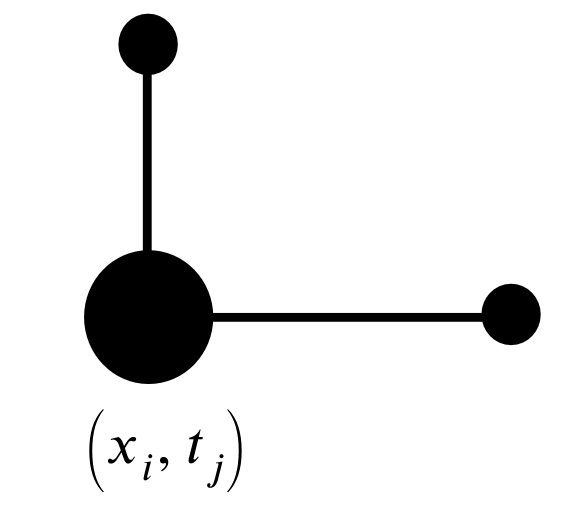
\includegraphics[scale=0.3]{images/img_12}
		 $$
		 Учитывая выбранный шаблон, мы можем заменить дифференциальные производные разностными и записать разностную схему в безиндексной форме
		 \begin{equation}
		 	\begin{cases}
		 	y_t + ay_x = 0,\ (x,t) \in \omega_{h\tau},\\
		 	y(x,0) = u_0(x),\ x \in \omega_h,
		 \end{cases}
		 \end{equation}
		 или что то же самое в индексной форме
		 $$\begin{dcases}
		 	\dfrac{y_k^{j+1}-y_k^j}{\tau} + a \dfrac{y_k^j - y_{k+1}^j}{h} = 0,\ k =0,\pm1,\ldots,\ j = 0,1,\ldots,\\
		 	y_k^0 = u_0(x_k),\ k =0,\pm1,\ldots.
		 \end{dcases}$$
		 Нужно вычислить погрешность аппроксимации разностной схемы. Учитывая тот факт, что разностная схема рассматривается для начального условия, то погрешность аппроксимации всей схемы будет определяться погрешностью аппроксимации начального условия. Поэтому для любой точки $(x,t) \in \omega_{h\tau}$ погрешность аппроксимации будет равна
		 $$\Psi(x,t) = u_t + au_x = \dfrac{\d u}{\d t} + \dfrac \tau 2 \dfrac{\d ^2 u}{\d t^2} + O(\tau^2) + a \left(\dfrac{\d u}{\d x} + \dfrac h 2 \dfrac{\d ^2 u}{\d x^2} + O(h^2) \right) = O(h+\tau).$$
		 Итак, учитывая вид погрешности, разностная схема имеет первый порядок аппроксимации по обеим переменным, то есть схема первого порядка.\\\\
		 После аппроксимации нам нужно исследовать эту схему на устойчивость. Для определенности используем метод разделения переменных для исследования на устойчивость. Подставим в разностную схему выражение
		 $$y_k^j = q^j e^{ik\varphi}$$
		 тогда получим
		 $$q = 1-\gamma(e^{i\varphi} -1),\ \gamma = \dfrac {a\tau}h.$$
		 Тогда
		 $$|q|^2 = (1-\gamma + \gamma \cos \varphi)^2 + \gamma^2 \sin^2 \varphi = 1 + 4 \gamma (1+\gamma)\sin ^2 \dfrac \varphi2.$$
		 Из этого выражения следует, что для любого $\varphi$ выполняется
		 $$|q^2|>1,$$
		 а следовательно схема будет неустойчивой для любых постоянных значений $\gamma$, если $a > 0$. Если положить $\gamma = O(h)$, то схема (2) будет устойчива на любом конечном промежутке (то есть наступит промежуток, на котором схему будет неустойчива). Если же $a < 0$, то разностная схема будет устойчива при выполнении условия $$-1 \leq \gamma \leq 0,$$
		 откуда следует, что $$|\gamma| = |a|\dfrac \tau h \leq 1.$$
		 После того, как мы определились с аппроксимацией и устойчивостью, нам нужно решить вопрос релазиации, то есть нахождения решения в любой точке сетки. Очевидно, что схему (2) можно реализовать по рекуррентной формуле вида
		 \begin{equation}
		 	\begin{cases}
		 	y_k^{j+1} = (1+\gamma)y_k^j - \gamma y_{k+1}^j,\ k = 0,\pm1,\ldots,\ j = 0,1,\ldots,\\
		 y_k^0 = u_0(x_k),\ k = 0,\pm 1
		 \end{cases}
		 \end{equation}
		 Формула (3) -- это еще одна запись схемы (2), однако по ней можно осуществить реализацию разностной схемы. Приближенное решение по формуле (3) может быть найдено послойно: начиная с нулевого временного слоя при $t=0$ ($j=0$) мы находим все $y_k^0$, а затем последовательно определяем $y_k^{j+1}$ по имеющимся $y_k^j$, $y_{k+1}^j$.
		 \\\\
		 $\bullet$ \textit{Разностные схемы, позволяющие получить приближенное решение по рекуррентным формулам называются \textbf{явными разностными схемами.}}\\\\
		 Явную разностную схему первого порядка можно построить и на другом шаблоне. Рассмотрим явную разностную схему, построенную на шаблоне
		 $$\text{Ш}(x,t) = \{(x,t),\ (x-h,t),\ (x,t+\tau)\}.$$
		 $$
		 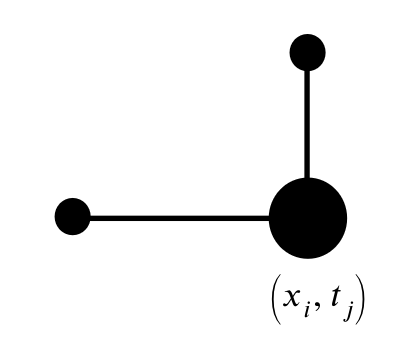
\includegraphics[scale=0.5]{images/img_11}
		 $$
		 \begin{equation}
		 	\begin{cases}
		 		y_t + ay_{\overline x} = 0,\ (x,t) \in \omega_{h\tau},\\
		 		y(x,0) = u_0(x),\ x \in \omega_h.
		 	\end{cases}
		 \end{equation}
		 Она будет также схемой первого порядка, а устойчивость мы исследовали ранее в примерах, то есть если $a>0$, то условием устойчивости является $$\gamma = \dfrac{a\tau}{h}\leq 1.$$ Если $a<0$, то схема (4) будет неустойчивой при $$\dfrac \tau h = \const.$$
		 Эта схема также является явной и может быть реализована аналогично схеме (2). Далее возникает вопрос, можно ли построить схемы более высокого порядка аппроксимации. Самый простой способ повышения порядка аппроксимации -- это расширение шаблона, при этом его можно расширять и по $x$ и по $t$. Но если мы будем расширять шаблон по $t$, то мы не сможем получить явные схемы, поэтому расширять шаблон мы будем только по $x$.\\\\
		 Рассмотрим шаблон, состоящий из четырех точек
		 $$\text{Ш}(x,t) = \{(x-h,t),\ (x,t),\ (x+h, t),\ (x,t+\tau)\}.$$
		 $$
		 	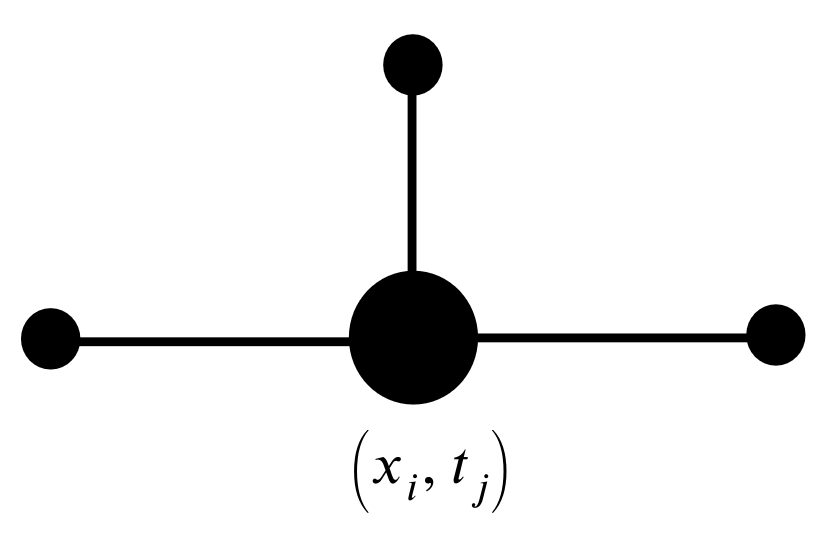
\includegraphics[scale=0.3]{images/img_13}
		 $$
		 Тогда разностная схема будет иметь вид
		 \begin{equation}
		 	\begin{cases}
		 		y_t + ay_{\overset{\circ}x} = 0,\ (x,t) \in \omega_{h\tau},\\
		 		y(x,0) = u_0(x),\ x \in \omega_h.
		 	\end{cases}
		 \end{equation}
		 Погрешность аппроксимации такой схемой есть величина
		 $$\Psi(x,t) = O(\tau + h^2).$$
		 Данная разностная схема является явной, так как $y_k^{j+1}$ мы можем найти по рекуррентной формуле
		 $$y_k^{j+1} = y_k^j - \gamma \dfrac{y_{k+1}^j - y_{k-1}^j}{2h}.$$
		 Если исследовать эту схему методом разделения переменных, то можно показать, что 
		 $$|q|^2 = 1 + \gamma ^2 \sin ^2 \varphi > 1,\ \forall \varphi, \ a \ne 0,$$
		 то есть при любых $\varphi$ и $a$ схема является неустойчивой. Таким образом, центральная разностная производная приводит нас к неустойчивым вычислениям.\\\\
		 Чтобы получить устойчивую разностную схему, подкорректируем ее. Значение $y_k^j$ заменим полусуммой значений в соседних точках шаблона
		 $$\dfrac 12 (y_{k+1}^j + y_{k-1}^j).$$
		 Теперь получим следующее разностное уравнение
		 \begin{equation}
		 	\dfrac{y_k^{j+1} - \frac 12 (y_{k+1}^j + y_{k-1}^j) }{\tau} + a \dfrac{y_{k+1}^j - y_{k-1}^j}{2h} = 0 
		 \end{equation}
		 Для уравнения (6) условия устойчивости по принципу максимума будут иметь следующий вид
		 $$\begin{cases}
		 	1+\gamma \geq 0,\\
		 	1 - \gamma \geq 0.
		 \end{cases}$$
		 Отсюда видно, что разностная схема (6) будет устойчивой при условии $|\gamma|\leq 1$ независимо от знака коэффициента $a$.\\\\
		 Но возникает вопрос, не была ли нарушена погрешность аппроксимации. Для ответа на этот вопрос определим погрешность аппроксимации для уравнения (6), для чего преобразуем его к виду
		 \begin{multline*}
		 	\psi(x_k, t_j) = u_t - \dfrac{h^2}{2\tau} u_{\ol x x} + a u_{\overset{\circ}x} = \dfrac{\d u}{\d t} + \dfrac \tau 2 \dfrac{\d ^2 u}{\d t^2} + O(\tau^2) - \dfrac {h^2}{2\tau} \left( \dfrac{\d ^2}{\d x^2} + O(h^2) \right) + a \left(\dfrac {\d u}{\d x} + O(h^2)\right)=\\
		 	=\left[ \dfrac{\d u}{\d t}+ a \dfrac{\d u}{\d x} = 0,\ \dfrac{\d^2 u}{\d t^2}= a^2 \dfrac{\d^2 u}{\d x^2}\right] = \left(\dfrac{a^2 \tau}{2} - \dfrac {h^2}{2\tau}\right)\dfrac{\d ^2u}{\d x^2} + O(\tau^2 + h^2 + \dfrac {h^4}\tau).
		 \end{multline*}
		 Таким образом, разностная схема (6) обладает условной аппроксимацией при условии $\dfrac {h^2}\tau \to 0$ при $h,\tau \to 0$. Если выбрать $\tau = O(h)$, то получим схему первого порядка, то есть $\psi = O(\tau + h)$. Если же выбрать $\tau = \dfrac h a$, то получим схему второго порядка, то есть
		 $\psi = O(\tau^2 + h^2)$.
		 \\\\
		 В заключение этого пункта приведем вариант явной разностной схемы, которая по свойству устойчивости совпадает со схемой (6), но обладает гарантированным вторым порядком аппроксимации
		 \begin{equation}
		 	\begin{cases}
		 		y_t + ay_{\overset{\circ}x} - \dfrac \tau 2 a^2 y_{\ol x x} = 0,\ (x,t) \in \omega_{h\tau},\\
		 		y(x,0) = u_0(x),\ x \in \omega_h
		 	\end{cases}
		 \end{equation}
		 $\bullet$ \textit{Разностная схема $(7)$ называется \textbf{разностной схемой Лакса-Вендроффора}.}
		 \subsection{Разностные схемы для краевой задачи.}
		 Рассмотрим краевую задачу для уравнения переноса
		 \begin{equation}
		 	\begin{cases}
		 		\dfrac{\d u}{\d t}+ a \dfrac{\d u}{\d x} = 0,\ t>0,\ 0 < x < \infty,\ a = \const \ne 0,\\
		 		u(x,0) = u_0(x),\ x \geq 0\\
		 		u(0,t) = \mu_0(t),\ t \geq 0.
		 	\end{cases}
		 \end{equation}
		 Для корректной постановки задачи необходимо выполнение условия согласования начального и граничного условий
		 $$u_0(0) = \mu_0(0).$$
		 Для задачи (8) известно точное решение
		 \begin{equation}
		 	u(x,t) = \begin{cases}
		 	u_0(x-at),\ t \leq \dfrac x a,\\
		 	\mu_0\left(t - \dfrac x a\right),\ t \geq \dfrac x a.
		 \end{cases}
		 \end{equation}
		 Для задачи (8) можно применять те же разностные схемы, что и для задачи (1). Но в случае краевой задачи также можно построить и неявные разностные схемы -- схемы, использующие на новом временном слое более одного значения приближенного решения.\\\\
		 Построим простейшую неявную разностную схему для задачи (8). Возьмем шаблон из трех точек
		 $$
		 	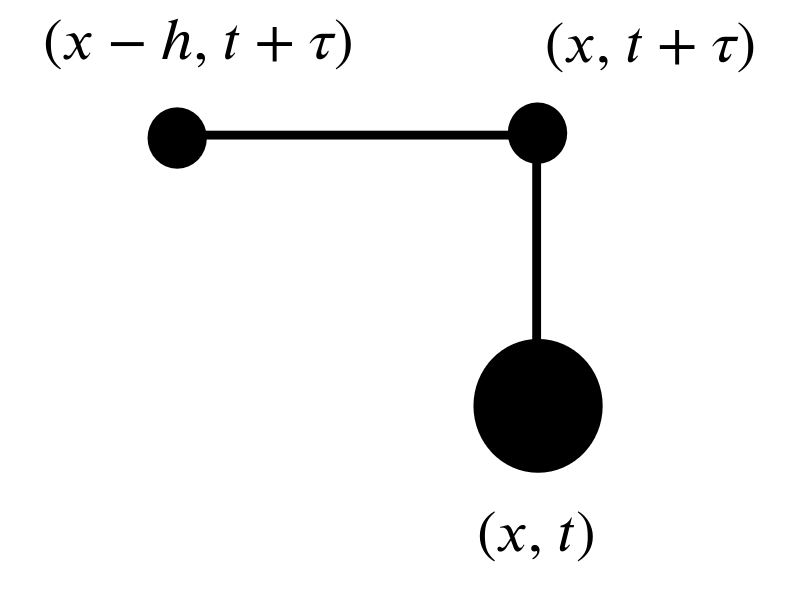
\includegraphics[scale=0.3]{images/img_14}
		 $$
		 Тогда для дифференциальной задачи (8) мы можем построить разностную задачу
		 \begin{equation}
		 	\begin{cases}
		 		y_t + a \hat y_{\ol x} =0,\ (x,t)\in \omega_{h\tau}\\
		 	y(x,0) = u_0(x),\ x \in \omega_h\\
		 	y(0,t) = \mu_0(t),\ t \in \omega_\tau.
		 	\end{cases}
		 \end{equation}
		 Символ $\hat{}$ означает значение функции в узле $t = t_j + \tau = t_{j+1}$. Для того чтобы применять разностную схему, нужно определить ее порядок аппроксимации и исследовать ее на устойчивость. Поэтому запишем первое уравнение в индексном виде
		 $$y_{k}^{j+1} = \dfrac{\gamma}{1+ \gamma} y_{k-1}^{j+1} + \dfrac{1}{1+\gamma}y_k^j, \gamma = \dfrac{a\tau}{h}.$$
		 При реализации сначала строятся значения из начального и граничного условий. То есть мы задаем $y_k^j$ при $j = 0$, $\forall k$, а затем при $k=0$, $\forall j$. Остальные значения функций можно вычислять по формуле выше. \\\\
		 Реализация этой схемы возможна двумя способами:
		 \begin{enumerate}
		 	\item по столбцам: начиная с точки $(x_1,t_0)$, последовательно вычисляем $y_1^j$, $j = \overline{0, j_0}$; затем берем $(x_k, t_0)$ и вычисляем $y_k^j$, $j = \ol{1,j_0}$;
		 	\item по строкам: сначала вычисляем $y_k^{j+1}$ при $j=0$, для всех $k = \ol{1, k_0}$, затем увеличиваем $j = 1,2,\ldots, j_0$ и повторяем вычисления.
		 \end{enumerate}
		 Второй случай чаще используется в практических вычислениях и носит название \textit{послойная реализация}. Далее для определенности мы будем рассматривать только послойную реализацию. Также второй способ на прямую связан с физическим смыслом задачи: мы имеем начальное распределение $u_0$, затем переходим на следующий слой $t+\tau$ и находим решение для всех $x$ и так далее.\\\\
		 Можно показать, что схема (10) обладает первым порядком аппроксимации, то есть $O(\tau + h)$. Кроме того данная схема при $a>0$ является абсолютно устойчивой, то есть при любых шагах $\tau$ и $h$ принцип максимума обеспечивает устойчивость по начальным данным. Таким образом, применение данной разностной схемы не накладывает никаких ограничений на узлы сетки.\\\\
		 Рассмотрим разностную схему, зависящую от параметра. Для этого рассмотрим шаблон из четырех точек 
		 $$
		 	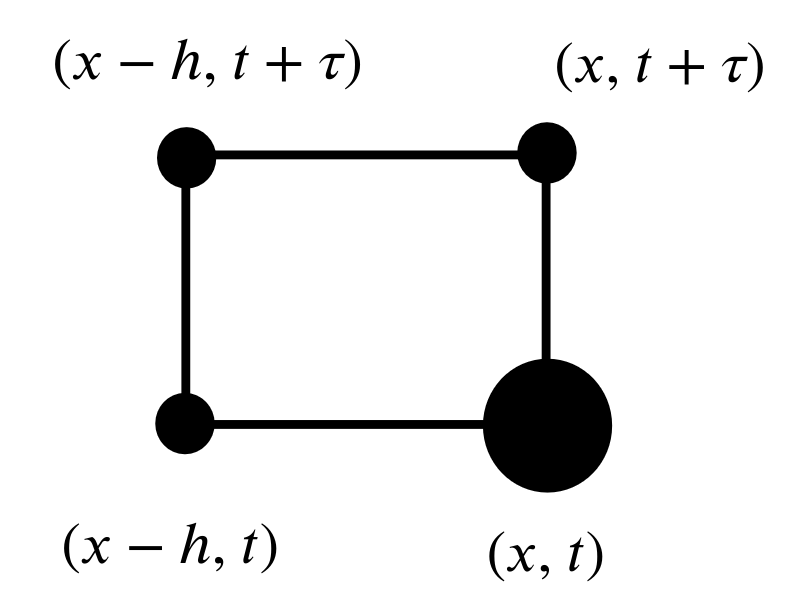
\includegraphics[scale=0.3]{images/img_15}
		$$
		На этом шаблоне запишем однопараметрическое семейство разностных схем вида
		\begin{equation}
			\begin{cases}
				y_t + a \hat (\sigma y_{\ol x} + (1-\sigma) y_{\ol x}) =0,\ (x,t)\in \omega_{h\tau}\\
				y(x,0) = u_0(x),\ x \in \omega_h\\
				y(0,t) = \mu_0(t),\ t \in \omega_\tau,
			\end{cases}
		\end{equation}
		где $\sigma$ -- это параметр, который иногда называют весом. Тогда разностную схему (11) можно назвать разностной схемой с весами. Легко видеть, что если $\sigma = 1$, то мы получим схему (10). Если $\sigma = 0$, то мы получим схему (4). Таким образом, мы рассматривали ранее частные случаи схемы с весами. \\\\
		Нас интересует точность и устойчивость этой разностной схемы. Получим выражение для погрешности аппроксимации этой разностной схемы, для этого введем обозначения
		$$\dot u = \dfrac{\d u(x,t)}{\d t},\ u' =\dfrac{\d u(x,t)}{\d x},\ \hat u = u(x, t+\tau).$$
		\section{Разностные схемы для уравнения теплопроводности.}
		\subsection{Исходная задача.}
		\subsection{Семейство шеститочечных разностных схем.}
		Обозначим через $\ol D$ область определения, и равномерную по каждому направлению сетку
		$$\ol\omega_{h\tau} = \ol \omega_h \times \ol \omega_\tau,\ \ol \omega_h = \{x_i = ih, i = \ol{0,N}, Nh = 1\}, \ \ol \omega_\tau = \{t_j = j\tau,j=\ol{0,N_1},\ N_1\tau=T\}.$$
		Таким образом, каждым узлом сетку является точка на плоскости с координатами $(x_i, t_j)$. Для аппроксимации исходного уравнения будем использовать шеститочечный шаблон
		((x,t) по центру, вправо, влево и вверх 3 точки).
		Для аппроксимации этой задачи на данном шаблоне будем рассматривать разностный оператор $L^{\sigma}_{h\tau}$, который был рассмотрен ранее в качестве примера. Таким образом, мы можем записать разностную задачу
		\begin{equation}
			\begin{cases}
				y_t = \Lambda(\sigma \hat y + (1-\sigma)y)+\varphi,\ (x,t)\in \omega_{h\tau},\\
				y(x,0) = u_0(x),\ x \in \ol \omega_h,\\
				y(0, t) = \mu_0(t),\ y(1,t) = \mu_1(t),\ t \in \ol \omega_\tau.
			\end{cases}
		\end{equation}
		Здесь $$\Lambda y = y_{\ol x x},\ \hat y = y(x, t+\tau),$$
		$\sigma$ -- это параметр, а $\varphi$ -- это сеточная функция, аппроксимирующая функцию $f$, определенную в задаче (1).\\\\
		$\bullet$ \textit{Разностная схема вида $(2)$ называется \textbf{семейством схем с весами}, или просто \textbf{схема с весами}.}
		\\\\
		Как и ранее будем пользоваться понятиями временного слоя и двухслойности схем.\\\\
		$\bullet$ \textit{\textbf{Временным слоем} (j-ым временным слоем) будем называть множество узлов сетки, лежащие на прямой $t = t_j$}.\\\\
		Рассмотрим вопрос реализации схемы с весами. Возьмем простейший случай $\sigma = 0$. Тогда шаблоном, аппроксимирующим задачу, будет являться четырехточечный шаблон вида ((x,t) по центру, влево, вправо. вверх). В этом случае получим разностное уравнение
		\begin{equation}
			y_t = y_{\ol x x} + \varphi.
		\end{equation}
		Тогда разностная схема $$\begin{cases}
				y_t = y_{\ol x x} + \varphi,\ (x,t)\in \omega_{h\tau}, \\
				y(x,0) = u_0(x),\ x \in \ol \omega_h,\\
				y(0, t) = \mu_0(t),\ y(1,t) = \mu_1(t),\ t \in \ol \omega_\tau.
		\end{cases}$$ будет называться \textit{явной разностной схемой}. Приближенное решение в каждой точке сетки может быть определено по следующему алгоритму:
		\begin{enumerate}
			\item решение на нулевом слое мы задаем в соответствии с начальным слоем
			\begin{equation}
				y_i^0 = u_0(x_i),\ i = \ol {0,N};
			\end{equation}
			\item строем решение на каждом слое последовательно, то есть для $j = \ol{0, N_1 - 1}$ определяем
			\begin{equation}
				y_0^{j+1} = \mu_0(t_{j+1}),\ y_i^{j+1} = y_i^j + \tau \left(\dfrac{y_{i-1}^j - 2 y_i^j + y_{i+1}^j}{h^2} + \varphi_i^j\right),\ i = \ol{1, N-1},\ y_N^{j+1} = \mu_1(t_{j+1}).
			\end{equation}
		\end{enumerate}
		Формулы (4) и (5) и определяют алгоритм реализации схемы с весами при $\sigma = 0$. \\\\
		Если $\sigma \ne 0$, то мы получим \textit{неявную разностную схему}. Расчеты по неявной схеме будут производиться уже на шеститочечном шаблоне, а вместо (3) у нас будет
		\begin{equation}
			y_t = \sigma \hat y_{\ol x x} + (1- \sigma)y_{\ol x x} + \varphi
		\end{equation}
		Тогда алгоритм реализации будет следующий:
		\begin{enumerate}
			\item нулевой слой заполняем по формуле (4);
			\item для всех $j = \ol {0, N_1-1}$ будем вычислять $y_i^j$, решая систему линейных алгебраических уравнений с трехдиагональной матрицей, а именно
			\begin{equation}
				\begin{dcases}
				\dfrac{\sigma}{h^2}y_{i-1}^{j+1} - \left(\dfrac{2\sigma}{h^2} + \dfrac 1 \tau\right) y_i^{j+1} + \dfrac {\sigma}{h^2} y_{i+1}^{j+1} = - F_i^j,\ i = \overline {1, N-1},\\
				y_0^{j+1} = \mu_0(t_{j+1}),\ y_N^{j+1} = \mu_1(t_{j+1}),
			\end{dcases}
			\end{equation}
			где $$F_i^j = \dfrac 1 \tau y_i^j + (1-\sigma) \dfrac{y_{i-1}^j - 2 y_i^j + y_{i+1}^j}{h^2} + \varphi_i^j.$$
		\end{enumerate}
		Очевидно, что наиболее эффективным методом решения системы (6) будет метод прогонки, а сам он будет устойчивый, что следует из вида коэффициентов.\\\\
		\textbf{Замечание.} Если взять $\sigma = 1$, то такая схема называется \textit{чисто неявной} (схема с опережением). Такая схема немного упрощает правую часть. Если взять $\sigma = \dfrac 12$, то такая схема называется \textit{симметричной схемой} (Кранка-Николсона).
		\subsection{Погрешность аппроксимации схем с весами.}
		Погрешность схемы с весами определим как разность между приближенным решением в точке сетки и точным решением в этой же точке
		$$z_i^j = y_i^j - u(x_i, t_j).$$
		Очевидно можно получить задачу для погрешности. Для этого подставим в (2) $$y_i^j = z_i^j + u(x_i, t_j)$$
		и получим разностную
		задачу для погрешности 
		\begin{equation}
			\begin{cases}
			z_t = \Lambda (\sigma \hat z + (1-\sigma)z) + \Psi,\ (x,t) \in \omega_{h\tau},\\
		z(x,0) = 0,\ x \in \ol \omega_h,\\
		z(0,t) = z(1,t) = 0,\ t \in \ol \omega_\tau,
		\end{cases}
		\end{equation}
		где $$\Psi = \Lambda(\sigma \hat u + (1-\sigma) u) - u_t + \varphi.$$
		Фактически в разностной задаче для погрешности (7) в качестве функции $\Psi$ выступает погрешность аппроксимации разностной схемы (2) на решении задачи (1).\\\\
		Оценив решение задачи (7) через функцию $\Psi$, можно доказать сходимость разностной схемы. При этом порядок сходимости будет связан с порядком малости величины $\Psi$.\\\\
		Исследуем погрешность аппроксимации разностной схемы, а значит оценим величину $\Psi$ в задаче (7).
		Для упрощения записи будем обозначать
		$$\dot u = \dfrac{\d u(x,t)}{\d t},\ u' =\dfrac{\d u(x,t)}{\d x}.$$ 
		Берем любую точку сетки $(x,t)$ и рассматриваем величину в этой точке
		\begin{multline*}
			\Psi(x,t) = \varphi + \sigma \left(\hat u '' + \dfrac{h^2}{12}\hat u '''' + O(h^4) \right) + (1-\sigma)\left(u'' + \dfrac {h^2}{12} u'''' + O(h^4)\right) - \left(\dot u + \dfrac \tau 2 \ddot u + O(\tau^2) \right)=\\
			= \varphi + \sigma \left(u'' + \tau \dot u '' + \dfrac {h^2}{12} u'''' + O(\tau^2 + h^4)\right) + (1-\sigma) \left(u'' + \dfrac{h^2}{12} u'''' + O(h^4)\right) - (\dot u - \dfrac \tau 2 \ddot u + O(\tau^2)) = \\=
			\varphi + (u'' - \dot u) + \sigma \tau \dot u '' + \dfrac {h^2}{12} u''' - \dfrac \tau 2 \ddot u + O(\tau^2 + h^4).
		\end{multline*}
		Учтем вид дифференциального оператора. По условию
		$$\dot u = u'' + f,\ \ddot u = \dot u '' + \dot f,\ \dot u '' = u'''' + f'',$$
		тогда получим выражение для аппроксимации разностной схемы
		$$\Psi(x,t) = \varphi - f + \tau \dot u''\left(\sigma - \dfrac 12 + \dfrac {h^2}{12\tau}\right) - \dfrac \tau 2 \dot f - \dfrac{h^2}{12}f'' + O(\tau^2 + h^4).$$
		\begin{enumerate}
			\item Пусть $\sigma$ -- это любое число. Если мы в качестве $\varphi$ выберем
			$$\varphi = f + O(\tau + h^2),$$ то тогда погрешность аппроксимации будет равна
			$$\Psi = O(\tau + h^2),\ u(x,t) \in C_2^4 (\ol D).$$
			\item Пусть $\sigma = \sigma_\alpha = \dfrac 12 + \alpha \dfrac{h^2}{\tau},$ где $\alpha$ -- любое число. Если в этом случае мы возьмем
			$$\varphi = f + \dfrac \tau 2 \dot f + O(\tau^2 + h^2) = f\left(x,t + \dfrac \tau 2\right) + O(\tau^2 + h^2).$$ Тогда мы получим значение погрешности равное
			$$\Psi = O(\tau^2 + h^2).$$
			Таким образом, мы получим семейство схем второго порядка. В частности при $\alpha = 0$ мы получим схему Кранка-Николсона.
			\item Пусть $\sigma = \sigma_* = \dfrac 12 - \dfrac {h^2}{12\tau}$, то есть мы выбрали $\alpha = - \dfrac {1}{12}$. Если мы возьмем
			$$\varphi = f + \dfrac \tau 2 \dot f + \dfrac{h^2}{12}f'' + O(\tau^2 + h^4),$$
			то получим порядок аппроксимации
			$$\Psi(x,t) = O(\tau^2 + h^4).$$
		\end{enumerate}
		В качестве $\varphi$ можно  выбирать также и разностные аппроксимации вместо производных, например,
		$$\varphi = f+\dfrac \tau 2 f_t + \dfrac{h^2}{12}f_{\ol x x}.$$
		Видно, что за счет выбора $\sigma$ мы можем получать разные схемы, обладающие разными свойствами точности.
		\subsection{Исследование устойчивости схемы с весами.}
		Не ограничивая общности исследование устойчивости схемы с весами будем проводить на задаче с однородными граничными условиями, а именно
		\begin{equation}
			\begin{cases}
				y_t = \Lambda(\sigma \hat y + (1-\sigma)y)+\varphi,\ (x,t)\in \omega_{h\tau},\\
				y(x,0) = u_0(x),\ x \in \ol \omega_h,\\
				y(0, t) = 0,\ y(1,t) = 0,\ t \in \ol \omega_\tau.
			\end{cases}
		\end{equation}
		Мы хотим исследовать на устойчивость решение $y$ задачи (9). \\\\
		$\bullet$ \textit{Разностная схема называется \textbf{устойчивой}, если для ее решения справедлива оценка}
		\begin{equation}
			\Norm{y(t)}_{(1)}\leq M_1 \Norm{u_0}_{(1)} + M_2 \underset{0 \leq t' \leq t}{\max}\Norm{\varphi(t')}_{(2)},\ t \in \omega_\tau
		\end{equation}
		В неравенстве $(10)$ $M_1$ и $M_2$ -- положительные константы, независящие от $\tau$ и $h$, а $\Norm{\cdot}_{(1)}$ и $\Norm{\cdot}_{(2)}$ -- это некоторые нормы на временном слое. \\\\
		Оказывается, если условие (10) выполняется, то по определенным ранее методам обеспечивается устойчивость решения. При $\varphi = 0$ оценка (10) принимает вид
		\begin{equation}
			\Norm{y(t)}_{(1)}\leq M_1 \Norm{u_0}_{(1)},\ t \in \omega_\tau
		\end{equation}
		Неравенство (11) выражает \textit{устойчивость по начальным данным}. Если $y(x,0) = 0$, то \begin{equation}
			\Norm{y(t)}_{(1)}\leq M_2 \underset{0 \leq t' \leq t}{\max}\Norm{\varphi(t')}_{(2)},\ t \in \omega_\tau.
		\end{equation}
		Неравенство (12) выражает \textit{устойчивость по правой части}.
		\\\\
		Для получения оценки (10) решение разностной задачи (9) представим в виде суммы
		\begin{equation*}
			y = \ol y + \ol{\ol y}, 
		\end{equation*}
		где $\ol y$ -- это решение однородного уравнения с ненулевым начальным условием, то есть в схеме (9) будет $\phi = 0$, $u_0 \ne 0$, а $\ol{\ol y}$ -- это решение неоднородного уравнения с нулевым начальным условием, то есть $\phi \ne 0$, $u_0 = 0$.
		\\\\
		Тогда, чтобы исследовать устойчивость решения разностной схемы нам нужно доказать по отдельности устойчивость для решения $\ol y$ (по начальным данным) и для $\ol{\ol y}$ (по правой части). 
		\subsubsection{Устойчивость по начальным данным.}
		Для функции $\ol y$ у нас имеется следующая задача
		\begin{equation}
			\begin{cases}
				\ol y_t = \Lambda(\sigma \hat{\ol{ y}} + (1-\sigma)\ol y),\ (x,t)\in \omega_{h\tau},\\
				\ol y(x,0) = u_0(x),\ x \in \ol \omega_h,\\
				\ol y(0, t) = 0,\ \ol y(1,t) = 0,\ t \in \ol \omega_\tau.
			\end{cases}
		\end{equation}
		Мы должны определить условие устойчивости данной задачи. Исследовать данную разностную схему на устойчивость будем методом разделения переменных. При этом, учитывая, что граничные условия задачи нулевые, мы разложим это решение по собственным функциям оператора разностной производной
		$$\Lambda y = y_{\ol x x},$$
		\begin{equation}
			y(x,t) = \sum_{k=1}^{N-1}T_k(t)\mu_k(x),
		\end{equation}
		где базисные функции \begin{equation*}
			\mu_k(x) = \sqrt 2 \sin (k \pi x).
		\end{equation*}
		$\bullet$ \textit{Функции вида $$y_k = T_k \mu _k$$ называются \textbf{$k$-ой гармоникой решения} $y(x,t)$.}\\\\
		Любая гармоника является решением задачи (13) при начальном условии $$u_0(x)= T_k(0)\mu_k(x).$$
		При этом как следует из принципа спектральной устойчивости, если схема устойчива по каждой гармонике, то она устойчива по начальным данным. Поэтому нам нужно лишь показать устойчивость по гармоникам. Подставим выражение (14) в (13), тогда получим соотношение
		\begin{equation*}
			\sum_{k=1}^{N-1} (T_k)_t \mu_k = \sum_{k=1}^{N-1} (\sigma \hat T_k + (1-\sigma)T_k)\Lambda \mu_k,
		\end{equation*}
		при этом
		$$\Lambda \mu_k = \lambda_k \mu _k,$$
		где $$\lambda_k = \dfrac{4}{h^2}\sin^2 \dfrac{k\pi h}{2}.$$
		Воспользуемся ортонормированностью системы функций $\mu_k$. Тогда из последнего равенства у нас останутся лишь слагаемые, относящиеся скалярному произведению при совпадающих индексах, то есть
		$$\dfrac{\hat T_k - T_k}{\tau} = -\lambda_k (\sigma \hat T_k + (1-\sigma)T_k),\ k=\overline{1, N-1}.$$
		Отсюда выразим $T_k$ на верхнем слое через $T_k$ на нижнем слое:
		\begin{equation}
			\hat T_k = q_k T_k,\ q_k = \dfrac{1 - (1-\sigma)\lambda_k \tau}{1+\sigma \lambda_k \tau},\ k = \ol {1, N-1}.
		\end{equation}
		Как следует из формулы (15) устойчивость $k$-ой гармоники будет иметь место при выполнении неравенства
		$$|q_k|\leq 1,$$
		отсюда следует, что 
		$$\sigma \geq \dfrac 12 - \dfrac{1}{\lambda_k \tau}.$$
		Нам нужно также оценить то, как себя ведут $\lambda_k$. Для собственных значений $\lambda_k$ справедлива оценка
		$$\lambda_k \leq \lambda _{N-1} < \dfrac{4}{h^2}.$$
		Отсюда следует, что 
		$$-\dfrac{1}{\lambda_k\tau} < -\dfrac{h^2}{4\tau}.$$
		Тогда условие устойчивости по начальным данным в сеточной норме $L_2$ будет выполняться, если 
		\begin{equation}
			\sigma \geq \sigma_0 = \dfrac 12 - \dfrac {h^2}{4\tau}.
		\end{equation}
		Рассмотрим некоторые частные случаи.
		\begin{enumerate}
			\item Если $\sigma = 0$, то схема будет явная и условие устойчивости имеет вид
			\begin{equation}
				\tau \leq \dfrac{h^2}{2}.
			\end{equation}
			$\bullet$ \textit{Условие $(17)$ это называется \textbf{условием Куранта задачи для уравнения теплопроводности}}.
			\item Если $\sigma \geq \dfrac 12$, то схема устойчива при любых шагах $\tau$ и $h$. В частности при $\sigma = 1$ мы получим чисто неявную схему, которая является абсолютно устойчивой для любых шагов $\tau, h$.
			\item Если $ 0 < \sigma < \dfrac 12$, то получим оценку
			\begin{equation}
				\tau \leq \dfrac{h^2}{2(1-\tau\sigma)}.
			\end{equation}
			\item Если $\sigma = \sigma_\alpha = \dfrac 12 + \alpha \dfrac {h^2}{\tau}$, то для выполнения условия устойчивости нужно взять $\alpha \geq -\dfrac 1 4$. Причем в данном случае схема будет устойчива при любых шагах $\tau$, $h$, а также она будет обладать порядком аппроксимации $O(\tau^2 + h^2)$.
			\item Если $\sigma = \sigma_* = \dfrac 12 - \dfrac{h^2}{12\tau}$, то схема будет устойчива при любых шагах $\tau$, $h$, а также будет обладать порядком аппроксимации $O(\tau^2 + h^4)$.
		\end{enumerate}
		\subsubsection{Устойчивость по правой части.}
		Для функции $\ol {\ol y}$ у нас имеется следующая задача
		\begin{equation}
			\begin{cases}
				\ol{\ol y_t} = \Lambda(\sigma \hat{\ol{ \ol y}} + (1-\sigma)\ol {\ol y})+\varphi,\ (x,t)\in \omega_{h\tau},\\
				\ol {\ol y}(x,0) = 0,\ x \in \ol \omega_h,\\
				\ol {\ol y}(0, t) = 0,\ \ol {\ol y}(1,t) = 0,\ t \in \ol \omega_\tau.
			\end{cases}
		\end{equation}
		Нам нужно исследовать устойчивость задачи (19). Вновь решение будем искать в виде формулы (14), но у нас также добавится сеточная функция в правой части основного уравнения. Поэтому мы представим эту сеточную функцию в виде разложения по системе базисных функций $\mu_k$
		$$\varphi(x,t) = \sum_{k=1}^{N-1}\varphi_k(t)\mu_k(x).$$
		Проделывая те же операции, как и в предыдущем пункте, мы можем получить соотношение между функциями $T_k$ на верхнем слое и на нижнем слое:
		\begin{equation}
			\hat T_k = q_k T_k + \dfrac{\tau \varphi_k}{1 + \sigma \lambda_k \tau}.
		\end{equation}
		Таким образом, суммируя по гармоникам, мы можем записать решение задачи (19) на верхнем слое
		$$\hat{\ol{\ol y}} = \sum_{k=1}^{N-1}\hat T_k \mu_k = \sum_{k=1}^{N-1}q_kT_k\mu_k + \tau \sum_{k=1}^{N-1}\dfrac{\varphi_k}{1 + \sigma \lambda_k \tau}\mu_k.$$
		Оценим это решение по норме
		\begin{multline*}
			\Norm {\hat{\ol{\ol y}}}\leq \Norm{\sum_{k=1}^{N-1}q_kT_k\mu_k } + \tau \Norm{ \sum_{k=1}^{N-1}\dfrac{\varphi_k}{1 + \sigma \lambda_k \tau}\mu_k} = \left[\Norm{\cdot} = \sqrt{(\cdot, \cdot )}\right]\leq \underset{1\leq k \leq N-1}{\max} |q_k| \left(\sum_{k=1}^{N-1}T_k^2\right)^{1/2} + \\ +
			\underset{1\leq k \leq N-1}{\max} \dfrac{\tau}{|1+\sigma \lambda_k \tau|} \left(\sum_{k=1}^{N-1}\phi_k^2\right)^{1/2} = \underset{1\leq k \leq N-1}{\max} |q_k|\cdot \Norm{\ol{\ol y}}  +
			\underset{1\leq k \leq N-1}{\max} \dfrac{\tau}{|1+\sigma \lambda_k \tau|} \Norm{\phi}.
		\end{multline*}
		Если одновременно будут выполняться условия $\sigma \geq \sigma_0$, $\sigma \geq 0$, то будет выполняться $1+\sigma \lambda_k \tau \geq 1$, $\forall k$ и $|q_k|\leq 1$. А тогда 
		$$\Norm {\hat{\ol{\ol y}}}\leq\Norm{\ol{\ol y}} + \tau \Norm{\varphi}.$$
		Если мы будем суммировать это неравенство по всем временным слоям, то мы получим оценку всего решения на любом слое 
		$$\Norm{\ol{\ol {y}^{j+1}}} \leq \Norm{y^0} + \tau \sum_{j'= 0}^j \Norm{\phi^{j'}}.$$
		Отсюда следует окончательная оценка
		\begin{equation}
			\Norm{\ol{\ol {y}^{j+1}}}\leq \Norm{\phi}_{\omega _{h\tau}}.
		\end{equation}
		Условие (21) доказывает устойчивость разностной схемы по правой части при одновременном выполнении условий $\sigma \geq \sigma_0$, $\sigma \geq 0$. \\\\
		Объединяя полученные результаты, и учитывая, что решение схемы (2) можно получить в виде суммы решений задач (13) и (19), можем сформулировать следующую теорему.
		\begin{theorem}
			Если выполнено условие $\sigma \geq \sigma_0$, $\sigma \geq 0$, то разностная схема с весами $(2)$ устойчива по начальным данным и правой части, и для ее решения справедлива оценка
			\begin{equation}
				\Norm{y^{j+1}}\leq \Norm{u_0} + \tau \sum_{j'=0}^j \Norm{\phi^{j'}}.
			\end{equation}
		\end{theorem}
		\textbf{Замечания.} \begin{enumerate}
			\item Если не требовать неотрицательности параметра $\sigma$, то можно показать, что условие устойчивости примет вид
		\begin{equation}
			\sigma \geq \sigma _\epsilon = \dfrac 12 - \dfrac{(1-\epsilon) h^2}{4\tau},\ \epsilon \in (0,1).
		\end{equation}
		Тогда вместо (22) у нас получится оценка вида
		\begin{equation}
			\Norm{y^{j+1}} \leq \Norm{u_0} + \dfrac \tau \epsilon \sum_{j'=0}^j \Norm{\phi^{j'}}.
		\end{equation}
		\item Если исследовать схему (2) на устойчивость по принципу максимума в норме $\Norm{\cdot}_C$, то условие устойчивости примет вид \begin{equation}
			\sigma \geq \dfrac 12 - \dfrac{h^2}{2\tau}.
		\end{equation}
		При этом при $\sigma = 0$ и $\sigma = 1$ оценки устойчивости по двум методам совпадают, а в остальных случаях эти оценки разные. Например, если $\sigma = \dfrac 12$, то в норме $\Norm{\cdot }_{L_2}$ схема является абсолютно устойчивой, а в норме $\Norm{\cdot }_C$ условно устойчивая при $\tau \leq h^2$.
		\end{enumerate}
		\subsection{Случай краевых условий третьего рода.}
		Пусть 
		\begin{equation}
			\dfrac{\d u(0,t)}{\d x} = \beta_0 u(0,t) - \mu_0(t),\ \beta_0 = \const > 0.
		\end{equation}
		В примере из п. 1.3 была получена аппроксимация краевого условия третьего рода с порядком $O(\tau + h^2)$. Применительно к (25) мы можем записать аппроксимацию
		$$\hat y_x (0,t) = \beta _0 y(0,t) + \dfrac h 2 y_t(0,t) - \tilde \mu_0(t),$$
		где $$\tilde \mu_0(t) = \mu_0(t) + \dfrac h2 f(0,t),\ t \in \omega_\tau$$
		на шаблоне (буква г).
		Легко видеть, что аналогичным порядком будет обладать аппроксимация
		$$y_x(0,t) = \beta_0 y(0,t) + \dfrac h2 y_t(0,t) - \tilde \mu_0(t), t \in \omega_\tau$$
		на шаблоне (вверх и вправо).\\\\
		Тогда можно составить аппроксимацию на четырехточечном шаблоне вида (квадратик,левый низ жирн) как линейную комбинацию двух аппроксимаций
		\begin{equation}
			y_x^{(\sigma)}(0,t) = \beta _0 y^{(\sigma)}(0,t) + \dfrac h2 y_t(0,t) - \tilde \mu_0(t),\ t \in \omega \tau,
		\end{equation}
		где $\sigma$ -- это числовой параметр, $$\tilde \mu_0(t) = \mu_0(t) + \dfrac h2 f(0,t),\ t \in \omega_\tau,$$
		а $$v^{(\sigma)} = \sigma \hat v + (1-\sigma v).$$
		Исследуем погрешность аппроксимации данного уравнения. Погрешность аппроксимации $\nu(0,t)$ будет обладать следующей аппроксимацией.
		\begin{enumerate}
			\item При любых $\sigma$ и
			$$\tilde \mu_0(t) = \mu_0(t) + \dfrac h2 f(0,t),$$
			получим $$\nu(0,t) = O(\tau + h^2).$$
			\item При любых $\sigma$ и
			$$\tilde \mu_0(t) = \mu_0(t) + \dfrac h2 f(0,t) + \sigma \tau \dot \mu_0(t),$$
			получим $$\nu(0,t) = O(\tau^2 + h^2).$$
			\item При $\sigma = \sigma_* = \dfrac 12 - \dfrac{h^2}{12\tau}$ и 
			$$\tilde \mu_0(t) = \mu_0(t) + \dfrac h2 f(0,t) + \left(\dfrac \tau 2 + \dfrac {h^2}{12}\right)\dot \mu_0(t) - \dfrac{h^2}{6}\beta_0 y_t(0,t) + \dfrac {h^2}{2}f'(0,t) + \dfrac{h^3}{24}f''(0,t) + \dfrac{\tau h}{4}\dot f(0,t)$$
			получим $$\nu(0,t) = O(\tau^2 + h^4).$$
		\end{enumerate}
		По аналогии с формулой (26) можно записать соответствующую аппроксимацию для краевого условия третьего рода на правой границе
		$$-\dfrac {\d u(1,t)}{\d x} = \beta_1 u(1,t) - \mu_1(t),\ \beta_1=\const > 0.$$
		В заключение отметим, что если $\beta _0 = \beta_1 = 0$, то мы получим условия второго рода, что упростит аппроксимацию. Следует иметь ввиду, что устойчивость разностной схемы с весами с краевыми условиями второго и третьего рода может быть исследована аналогично тому, как было изложено выше.
		\end{document}




